\chapter{Stetigkeit}

\setcounter{section}{6}
\setcounter{subsection}{0}
\setcounter{subsubsection}{1}
\setcounter{secnumdepth}{3}
\subsection{Stetigkeit (Definition)}
\href{https://youtu.be/w5zo40vnyRQ}{Video 01}\\
Sei $ f:\mathbb{D}_f\longmapsto \mathbb{W}_f $ Funktion und $ x_0\in \mathbb{D}_f $\\
Definition:\\
Die Funktion $ f $ heißt in $ x_0\in\mathbb{D}_f $ stetig, wenn $ \lim\limits_ {x\to x_0}f(x)=f(x_0) $\\
\begin{align*}
\Leftrightarrow \lim\limits_ {\substack{x\to x_0\\x<0}}f(x)=f(x_0)=\lim\limits_ {\substack{x\to x_0\\x>0}}f(x)=f(x_0)
\end{align*}
\begin{center}
	Die Folge $ (a_n)$ bzw. $f(a_n) $ kommt von links zum Wert $ x_0$ bzw.$f(x_0) $\\ und rechts zum Wert $ x_0$ bzw. $f(x_0) $.\\
	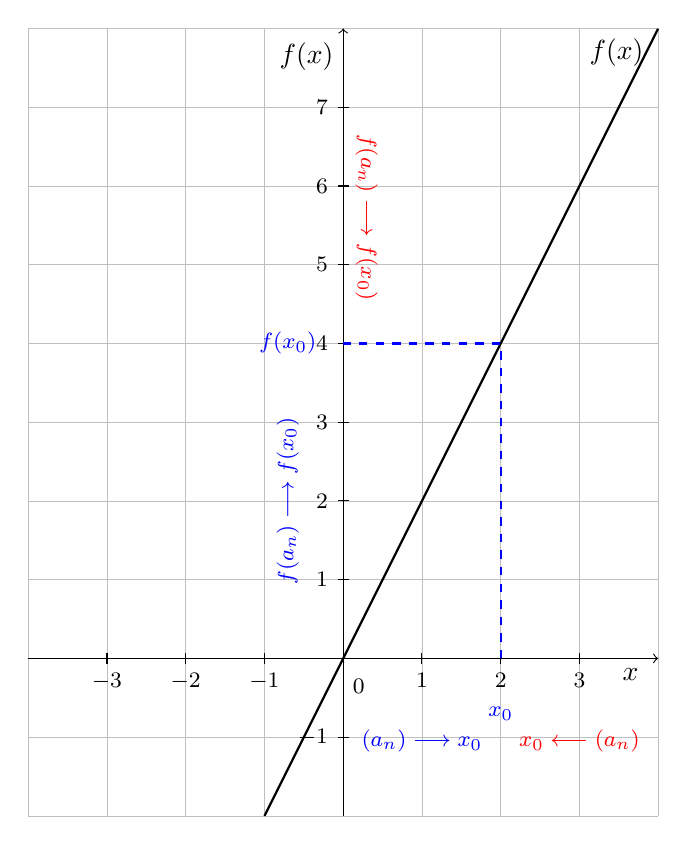
\begin{tikzpicture}
	
	% Gitternetzlinien
	\draw[xstep=1cm, ystep=1cm, very thin, color=lightgray] (-4,8) grid (4,-2);
	% x-Achse
	\draw[->] (-4,0) -- (4,0) node[below,xshift=-1em] {$x$}; 
	%Zahlen auf x-Achse
	\foreach \x in {-3,...,-1}
	\draw[shift={(\x,0)},color=black] (0pt,2pt) -- (0pt,-2pt) node[below] {\footnotesize $\x$};
	\foreach \x in {1,...,3}
	\draw[shift={(\x,0)},color=black] (0pt,2pt) -- (0pt,-2pt) node[below] {\footnotesize $\x$};
	% y-Achse 
	\draw[->] (0,-2) -- (0,8) node[left,yshift=-1em] {$f(x)$};%node[above left]
	%Zahlen auf y-Achse
	\foreach \y in {-1,...,-1}
	\draw[shift={(0,\y)},color=black] (2pt,0pt) -- (-2pt,0pt) node[left] {\footnotesize $\y$};
	\foreach \y in {1,...,7}
	\draw[shift={(0,\y)},color=black] (2pt,0pt) -- (-2pt,0pt) node[left] {\footnotesize $\y$};
	%Ursprung
	\draw[color=black] (0pt,-10pt) node[right] {\footnotesize $0$};
	
	
	
	\draw[thick,color=black] plot[samples=200, domain=-1:4] 
	(\x,{2*\x}) node[below, xshift=-1.5em]{$f(x)$};
	
	\draw[color=blue] (2,0) node[yshift=-20] {\footnotesize $x_0$};
	\draw[color=blue] (1,0) node[yshift=-30] {\footnotesize $(a_n)\longrightarrow x_0$};
	\draw[color=blue] (0,4) node[xshift=-20] {\footnotesize $f(x_0)$};
	\draw[color=blue] (0,2) node[xshift=-20,rotate=90] {\footnotesize $f(a_n)\longrightarrow f(x_0)$};
	\draw[color=blue,dashed,thick] (2,0)--(2,4)--(0,4);
	\draw[color=red] (3,0) node[yshift=-30] {\footnotesize $x_0\longleftarrow (a_n)$};
	\draw[color=red] (1,5.6) node[xshift=-20,rotate=-90] {\footnotesize $f(a_n)\longrightarrow f(x_0)$};
	\end{tikzpicture}\\
\end{center}
Beispiel:\\
Sei $ f:\mathbb{R}\longmapsto[0,\infty[ $ mit $ f(x)=x^2 $\\
\textbullet\;\; Wenn $ f(x) $ ist stetig bei $ x_0=0 $, dann ist $ f(x) $ stetig im Punkt $ x_0 $.\\
\begin{quote}
	\begin{align*}
	\lim\limits_ {\substack{x \to 0\\x<0}}f(x)=	\lim\limits_ {\substack{x \to 0\\x<0}}x^2=\underbrace {0}_{f(0)=0^2}=\lim\limits_ {\substack{x \to 0\\x>0}}f(x)=	\lim\limits_ {\substack{x \to 0\\x>0}}x^2
	\end{align*}
	
\end{quote}
\textbullet\;\; Wenn $ f(x) $ ist stetig bei jeden Wert von $ x_0\in\mathbb{D}_f$, dann heißt $ f(x) $ ist stetig.\\
\begin{quote}
	\begin{align*}
	\lim\limits_ {\substack{x \to x_0\\x<0}}f(x)=	\lim\limits_ {\substack{x \to x_0\\x<0}}x^2=\underbrace {x_0^2}_{f(x_0)=x_0^2}=\lim\limits_ {\substack{x \to x_0\\x>0}}f(x)=	\lim\limits_ {\substack{x \to x_0\\x>0}}x^2
	\end{align*}
	
	
\end{quote}
\subsubsection{Unstetigkeit-Teil I}
\href{https://youtu.be/KsP333nJ9PY}{Video 02}\\
Die Funktion $ f:\mathbb{D}_f\longmapsto\mathbb{W}_f $ heißt in $ x_0 \in \mathbb{D}_f $ unstetig , wenn $ f $ in $ x_0 $ nicht stetig ist.\\
Wenn die Funktion in einem Punkt $ x_0 $ nicht stetig ist, dann ist die ganze Funktion nicht stetig.\\
\begin{align*}
\boxed{\lim\limits_ {\substack{x\to x_0\\x<x_0}}f(x)=\lim\limits_ {\substack{x\to x_0\\x>x_0}}f(x)=f(x_0)}
\end{align*}
\textbf{Typ 1: Lücke}\\
\begin{align*}
&\text{Grenzwerte exestieren }\\
&\boxed{\lim\limits_ {\substack{x\to x_0\\x<x_0}}f(x)=\lim\limits_ {\substack{x\to x_0\\x>x_0}}f(x)\neq f(x_0)}
\end{align*}
Bemerkung: Grenzwert muß ein reeller Wert sein:\vspace*{2mm}\\
Beispiel:\\
Sei: $ f:\mathbb{R}\longmapsto \mathbb{R} $ mit $ f(x) =     \left\{ \begin{array}{rcl}
x^2& \mbox{für} & x\neq0\\
1& \mbox{für} & x= 0 \\

\end{array}\right. $\\
\begin{center}
	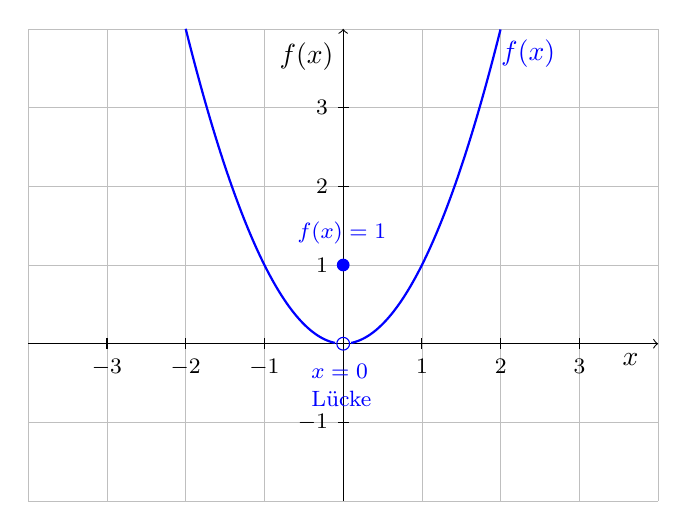
\begin{tikzpicture}
	
	% Gitternetzlinien
	\draw[xstep=1cm, ystep=1cm, very thin, color=lightgray] (-4,4) grid (4,-2);
	% x-Achse
	\draw[->] (-4,0) -- (4,0) node[below,xshift=-1em] {$x$}; 
	%Zahlen auf x-Achse
	\foreach \x in {-3,...,-1}
	\draw[shift={(\x,0)},color=black] (0pt,2pt) -- (0pt,-2pt) node[below] {\footnotesize $\x$};
	\foreach \x in {1,...,3}
	\draw[shift={(\x,0)},color=black] (0pt,2pt) -- (0pt,-2pt) node[below] {\footnotesize $\x$};
	% y-Achse 
	\draw[->] (0,-2) -- (0,4) node[left,yshift=-1em] {$f(x)$};%node[above left]
	%Zahlen auf y-Achse
	\foreach \y in {-1,...,-1}
	\draw[shift={(0,\y)},color=black] (2pt,0pt) -- (-2pt,0pt) node[left] {\footnotesize $\y$};
	\foreach \y in {1,...,3}
	\draw[shift={(0,\y)},color=black] (2pt,0pt) -- (-2pt,0pt) node[left] {\footnotesize $\y$};
	%Ursprung
	\draw[color=blue] (-15pt,-20pt) node[right] {\footnotesize Lücke};
	\draw[color=blue] (-15pt,-10pt) node[right] {\footnotesize $x=0$};
	\draw[color=blue] (-20pt,40pt) node[right] {\footnotesize $f(x)=1$};
	\draw[thick,color=blue] plot[samples=200, domain=-2:-0.1] 
	(\x,{\x*\x});
	
	\draw[thick,color=blue] plot[samples=200, domain=0.1:2] 
	(\x,{\x*\x}) node[below, xshift=1em]{$f(x)$};
	
	\draw [blue] (0,0) circle (.081cm) ;
	\fill [blue] (0,1) circle (.081cm) ;	
	\end{tikzpicture}\\
\end{center}
Wenn der linksseitige Grenzwert bei $ x_0 $ und der rechtsseitige Grenzwert bei $ x_0 $ gleich ist und der Funktionswert nicht gleich den Grenzwert ist, dann spricht man von einer Lücke.\\
Es gilt:\\
\begin{align*}
&\lim\limits_ {\substack{x \to 0\\x<0}}f(x)=0=\lim\limits_ {\substack{x \to 0\\x>0}}f(x)\neq f(x_0)=f(0)=1\\
&\Rightarrow\;\;f\;\text{ist in  }\;x_0=0\;\;\text{nicht stetig}
\end{align*}
Da der linksseitige und der rechtsseitige Grenzwert gleich ist und der Funktionswert nicht gleich dem Grenzwert  an der Stelle $ x_0 $  ist, ist die Funktion nicht stetig und besitzt eine behebbare Lücke.\\
Bemerkung:\\
In diesen Fall kann man die Unstetigkeit beheben.\\
Z.B. ist die Funktion $ \overset{\AC}{f}:\mathbb{R}\longmapsto \mathbb{R}$  mit $ f(x) =     \left\{ \begin{array}{rcl}
x^2 & \mbox{für} & x\neq0\\
0 & \mbox{für} & x= 0 \\

\end{array}\right.$ stetig.\\
Damit ist die Unstetigkeitsstelle behoben.\\
Die Funktion $ \overset{\AC}{f}$ ist gleich die stetige Fortsetzung von $ f $.\vspace*{6mm}\\
Es ist eigentlich nicht notwendig, dass $ x_0 $ in $ \mathbb{D}_f $ ist.\\
Sei: $ f:\mathbb{R}\backslash \{0\}\longmapsto\mathbb{R} $ mit $ f(x)=x^2 $\\
\begin{center}
	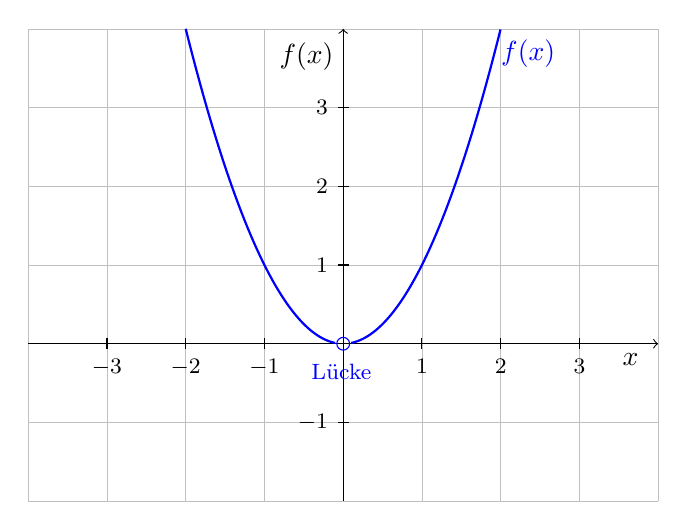
\begin{tikzpicture}
	
	% Gitternetzlinien
	\draw[xstep=1cm, ystep=1cm, very thin, color=lightgray] (-4,4) grid (4,-2);
	% x-Achse
	\draw[->] (-4,0) -- (4,0) node[below,xshift=-1em] {$x$}; 
	%Zahlen auf x-Achse
	\foreach \x in {-3,...,-1}
	\draw[shift={(\x,0)},color=black] (0pt,2pt) -- (0pt,-2pt) node[below] {\footnotesize $\x$};
	\foreach \x in {1,...,3}
	\draw[shift={(\x,0)},color=black] (0pt,2pt) -- (0pt,-2pt) node[below] {\footnotesize $\x$};
	% y-Achse 
	\draw[->] (0,-2) -- (0,4) node[left,yshift=-1em] {$f(x)$};%node[above left]
	%Zahlen auf y-Achse
	\foreach \y in {-1,...,-1}
	\draw[shift={(0,\y)},color=black] (2pt,0pt) -- (-2pt,0pt) node[left] {\footnotesize $\y$};
	\foreach \y in {1,...,3}
	\draw[shift={(0,\y)},color=black] (2pt,0pt) -- (-2pt,0pt) node[left] {\footnotesize $\y$};
	%Ursprung
	\draw[color=blue] (-15pt,-10pt) node[right] {\footnotesize Lücke};
	%\draw[color=blue] (-20pt,40pt) node[right] {\footnotesize $f(x)=1$};
	\draw[thick,color=blue] plot[samples=200, domain=-2:-0.1] 
	(\x,{\x*\x});
	
	\draw[thick,color=blue] plot[samples=200, domain=0.1:2] 
	(\x,{\x*\x}) node[below, xshift=1em]{$f(x)$};
	
	\draw [blue] (0,0) circle (.081cm) ;
	%\fill [blue] (0,1) circle (.081cm) ;	
	\end{tikzpicture}\\
\end{center}

\begin{align*}
\lim\limits_ {\substack{x \to 0\\x<0}}f(x)=0=\lim\limits_ {\substack{x \to 0\\x>0}}f(x)\neq f(0) \;\;\text{nicht im Definitionbereich, hier ist eine Lücke }
\end{align*}
In diesen Fall kann man die Unstetigkeit beheben mit:\\
\begin{align*}
f(x) =     \left\{ \begin{array}{rcl}
x^2& \mbox{für} & x\neq0\\
0 & \mbox{für} & x= 0 \\
\end{array}\right.
\end{align*}
\textbf{Typ 2: Sprungstelle}\\
\begin{align*}
\text{Grenzwerte exestieren }\\
\boxed{\lim\limits_ {\substack{x\to x_0\\x<x_0}}f(x)\neq\lim\limits_ {\substack{x\to x_0\\x>x_0}}f(x)}
\end{align*}
Beispiel:\\
Sei: $ f:\mathbb{R}\longmapsto\mathbb{R} $ mit$ f(x) =     \left\{ \begin{array}{rcl}
1 & \mbox{für} & x\geq0\\
-1 & \mbox{für} & x< 0 \\

\end{array}\right.$\\
\begin{center}
	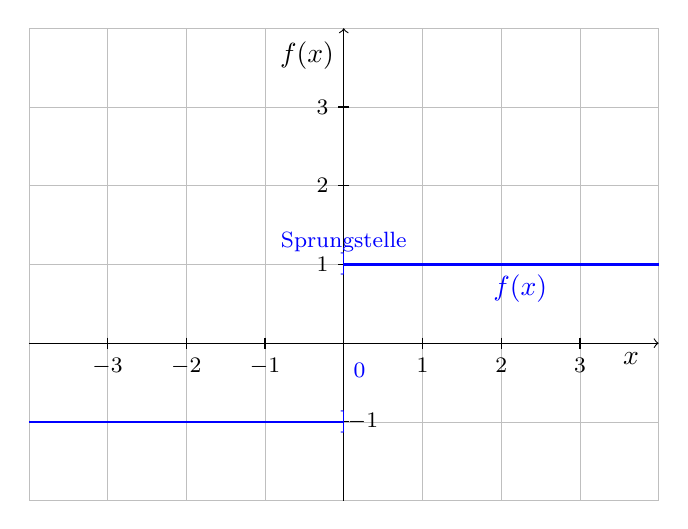
\begin{tikzpicture}
	
	% Gitternetzlinien
	\draw[xstep=1cm, ystep=1cm, very thin, color=lightgray] (-4,4) grid (4,-2);
	% x-Achse
	\draw[->] (-4,0) -- (4,0) node[below,xshift=-1em] {$x$}; 
	%Zahlen auf x-Achse
	\foreach \x in {-3,...,-1}
	\draw[shift={(\x,0)},color=black] (0pt,2pt) -- (0pt,-2pt) node[below] {\footnotesize $\x$};
	\foreach \x in {1,...,3}
	\draw[shift={(\x,0)},color=black] (0pt,2pt) -- (0pt,-2pt) node[below] {\footnotesize $\x$};
	% y-Achse 
	\draw[->] (0,-2) -- (0,4) node[left,yshift=-1em] {$f(x)$};%node[above left]
	%Zahlen auf y-Achse
	\foreach \y in {-1,...,-1}
	\draw[shift={(0,\y)},color=black] (2pt,0pt) -- (-2pt,0pt) node[right] {\footnotesize $\y$};
	\foreach \y in {1,...,3}
	\draw[shift={(0,\y)},color=black] (2pt,0pt) -- (-2pt,0pt) node[left] {\footnotesize $\y$};
	%Ursprung
	\draw[color=blue] (0pt,-10pt) node[right] {\footnotesize $0$};
	
	\draw[thick,color=blue] plot[samples=200, domain=0:4] 
	(\x,{1}) node[below, xshift=-5em] {$f(x)$};
	
	\draw[thick,color=blue] plot[samples=200, domain=-4:0] 
	(\x,{-1});
	\draw[color=blue,thick] (0pt,-1) node[xshift=0em] {\footnotesize $]$};
	
	\draw[thick,color=blue] (0pt,1) node[xshift=0em] {\footnotesize $]$};
	\draw[thick,color=blue] (0pt,1) node[xshift=0em,yshift=0.8em] {\footnotesize Sprungstelle};
	\end{tikzpicture}\\
\end{center}
Betrachte: für $ x_0=0 $\\
\begin{align*}
\lim\limits_ {\substack{x \to 0\\x<0}}f(x)=-1\neq\lim\limits_ {\substack{x \to 0\\x\geq0}}f(x)=1
\end{align*}
\subsubsection{Unstetigkeit-Teil II}
\href{https://youtu.be/8bunAaehx4A}{Video 03}\\
\textbf{Typ 3: Polstelle}\\
\begin{align*}
\boxed{\lim\limits_ {\substack{x\to x_0\\x<x_0}}f(x)=\pm\infty\;\;\text{oder }\lim\limits_ {\substack{x\to x_0\\x>x_0}}f(x)=\pm\infty}
\end{align*}
Beispiel:\\
Sei: $ f:\mathbb{R}\longmapsto\mathbb{R} $ mit$ f(x) =     \left\{ \begin{array}{rcl}
\frac{1}{x} & \mbox{für} & x>0\\
0 & \mbox{für} & x\leq0 \\

\end{array}\right.$\\
\begin{center}
	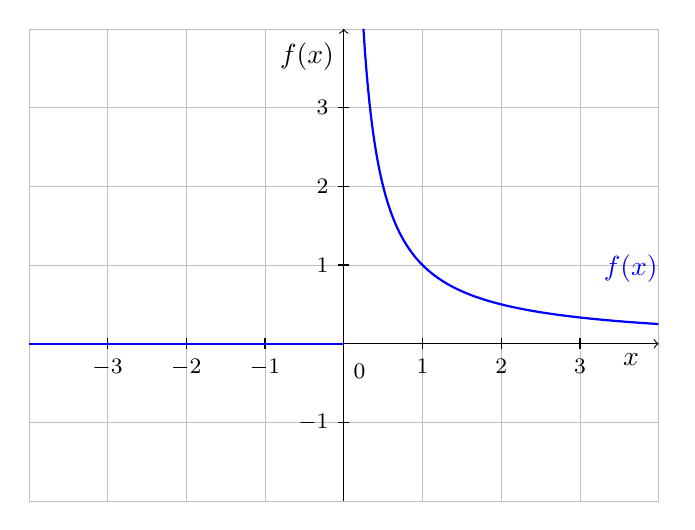
\begin{tikzpicture}
	
	% Gitternetzlinien
	\draw[xstep=1cm, ystep=1cm, very thin, color=lightgray] (-4,4) grid (4,-2);
	% x-Achse
	\draw[->] (-4,0) -- (4,0) node[below,xshift=-1em] {$x$}; 
	%Zahlen auf x-Achse
	\foreach \x in {-3,...,-1}
	\draw[shift={(\x,0)},color=black] (0pt,2pt) -- (0pt,-2pt) node[below] {\footnotesize $\x$};
	\foreach \x in {1,...,3}
	\draw[shift={(\x,0)},color=black] (0pt,2pt) -- (0pt,-2pt) node[below] {\footnotesize $\x$};
	% y-Achse 
	\draw[->] (0,-2) -- (0,4) node[left,yshift=-1em] {$f(x)$};%node[above left]
	%Zahlen auf y-Achse
	\foreach \y in {-1,...,-1}
	\draw[shift={(0,\y)},color=black] (2pt,0pt) -- (-2pt,0pt) node[left] {\footnotesize $\y$};
	\foreach \y in {1,...,3}
	\draw[shift={(0,\y)},color=black] (2pt,0pt) -- (-2pt,0pt) node[left] {\footnotesize $\y$};
	%Ursprung
	\draw[color=black] (0pt,-10pt) node[right] {\footnotesize $0$};
	
	\draw[thick,color=blue] plot[samples=200, domain=0.25:4] 
	(\x,{1/\x}) node[xshift=-1em,yshift=20] {$f(x)$};
	
	\draw[thick,color=blue] plot[samples=200, domain=-4:0] 
	(\x,{0});
	
	
	
	\end{tikzpicture}\\
	\glqq Ist auch eine unendliche Sprungstelle.\grqq\\
\end{center}
\begin{align*}
&\lim\limits_ {\substack{x \to 0\\x<0}}f(x)=0\;\;\;\;\lim\limits_ {\substack{x \to 0\\x>0}}f(x)=\infty\\
&\Rightarrow f\;\;\text{in }\;\; x_0=0\;\;\text{unstetig }\\
&\text{d.h. }\;\;f\;\;\text{ist nicht stetig }\\
\end{align*}
\textbf{Typ 3: Oszillation}\\
\begin{center}
	\fbox{\parbox  {78mm} {
			$\lim\limits_ {\substack{x \to 0\\x<0}}f(x)$ existiert nicht und $\lim\limits_ {\substack{x \to 0\\x<0}}f(x)\neq\infty$\vspace*{4mm}\\
			$\lim\limits_ {\substack{x \to 0\\x>0}}f(x)$ existiert nicht und $\lim\limits_ {\substack{x \to 0\\x>0}}f(x)\neq\infty$\\}}
\end{center}
Beispiel:\\
Sei: $ f:\mathbb{R}n\longmapsto\mathbb{R}n $ mit $ f(x) =     \left\{ \begin{array}{rcl}
\sin(\frac{1}{x}) & \mbox{für} & x\neq0\\
0 & \mbox{für} & x=0 \\

\end{array}\right. $\\
\begin{center}
	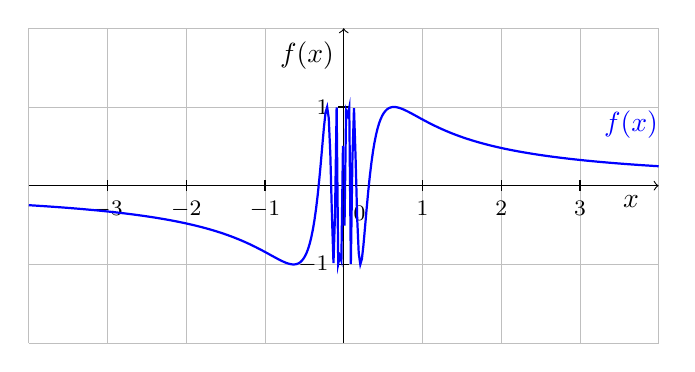
\begin{tikzpicture}
	
	% Gitternetzlinien
	\draw[xstep=1cm, ystep=1cm, very thin, color=lightgray] (-4,2) grid (4,-2);
	% x-Achse
	\draw[->] (-4,0) -- (4,0) node[below,xshift=-1em] {$x$}; 
	%Zahlen auf x-Achse
	\foreach \x in {-3,...,-1}
	\draw[shift={(\x,0)},color=black] (0pt,2pt) -- (0pt,-2pt) node[below] {\footnotesize $\x$};
	\foreach \x in {1,...,3}
	\draw[shift={(\x,0)},color=black] (0pt,2pt) -- (0pt,-2pt) node[below] {\footnotesize $\x$};
	% y-Achse 
	\draw[->] (0,-2) -- (0,2) node[left,yshift=-1em] {$f(x)$};%node[above left]
	%Zahlen auf y-Achse
	\foreach \y in {-1,...,-1}
	\draw[shift={(0,\y)},color=black] (2pt,0pt) -- (-2pt,0pt) node[left] {\footnotesize $\y$};
	\foreach \y in {1,...,1}
	\draw[shift={(0,\y)},color=black] (2pt,0pt) -- (-2pt,0pt) node[left] {\footnotesize $\y$};
	%Ursprung
	\draw[color=black] (0pt,-10pt) node[right] {\footnotesize $0$};
	
	\draw[thick,color=blue,rotate=180] plot[samples=200, domain=0.01:4] 
	(\x,{sin(1/\x r)});
	
	\draw[thick,color=blue] plot[samples=200, domain=0.01:4] 
	(\x,{sin(1/\x r)}) node[xshift=-1em,yshift=1.5em]{$f(x)$};
	
	
	\end{tikzpicture}\\
\end{center}
\begin{align*}
\lim\limits_ {\substack{x \to 0\\x<0}}f(x)=\lim\limits_ {\substack{x \to 0\\x<0}} \sin(\frac{1}{x})\text{existiert nicht! };\;\\
\lim\limits_ {\substack{x \to 0\\x>0}}f(x)=\lim\limits_ {\substack{x \to 0\\x<0}} \sin(\frac{1}{x})\text{existiert nicht! };\;\\
\end{align*}
Der Funktionswert ist immer zwischen -1 und +1 (ähnlich wie $ \lim\limits_ {n\to\infty}(-1)^n $)und der Grenzwert von dem Funktionswert existiert nicht.\\
\begin{align*}
&-1\leq\lim\limits_ {\substack{x \to 0\\x<0}}f(x)=\lim\limits_ {\substack{x \to 0\\x<0}}\leq 1 \;\;\text{und }\lim\limits_ {\substack{x \to 0\\x<0}}f(x)\;\;\text{existiert nicht }\\
&\Rightarrow f \;\;\text{in }\;\;x_0=0\;\;\text{nicht stetig ist. }
\end{align*}
Bemerkung:\\

\textbullet\;\;Typ 2-4 sind nicht behebbar\\

\textbullet\;\;Polynome und rationale Funktionen sind auf ihren Definitionsbereich stetig.\\

\textbullet\;\;Stetigkeitsuntersuchungen werden immer auf zusammengesetzte Funktionen angewandt.\\

\subsection{Rechenregeln für stetge Funktionen}
\href{https://youtu.be/hV8uqmwoxiI}{Video 04}\\
Seien $ f,g $ stetige Funktionen, dann sind\\
\begin{center}
	\fbox{\parbox  {70mm} {\textbullet \;\;$ f+g, f\cdot g, f-g $\vspace*{2mm}\\
			\textbullet \;\; $ \frac{f}{g} $ für $ g(x)\neq 0 $\vspace*{2mm}\\\textbullet \;\;$ f\circ g $, wenn $ f\circ g  $ wohldefiniert ist}}\vspace*{4mm}\\
	stetige Funktionen.
\end{center}
Beispiel:\\
Überprüfe ob:\\
\begin{align*}
|.|:\mathbb{R}\longmapsto \mathbb{R} [0,\infty[\;\;\text{mit }\;\;|x| =     \left\{ \begin{array}{rcl}
-x & \mbox{für} & x<0\\
x & \mbox{für} & x\geq 0 \\
\end{array}\right.\;\;\text{stetig ist. }
\end{align*}
Da der Betrag $ |.| $ für $ x\in \;\; ]-\infty,0[ $ und $ x\in \;\; [0,\infty[  $ als Komposition einer stetigen Abbildung ist, bleibt nur noch die Stelle $ x_0 $ zur Prüfung übrig.\\
Bemerkung: Dies in der Prüfung hinschreiben, sonst gibt es Punktabzug!\\
\begin{align*}
\lim\limits_ {\substack{x\to 0\\x<0}}|x|=\lim\limits_ {x\to 0}-x=0=|0|=\lim\limits_ {\substack{x\to 0\\x>0}}|x|=\lim\limits_ {x\to\ 0}x=0\\
\end{align*}
D.h. der $ |.| $ ist stetig.\\
\subsubsection{Aufgabe 1 zu Rechenregeln von stetigen Funktionen}
\href{https://youtu.be/0dB1Z7ZqMlk}{Video 08}\\
Untersuche folgende Funktion auf Stetigkeit:\\
\begin{align*}
f:\mathbb{R}\longmapsto \mathbb{R}\;\;\text{mit }\;\;f(x):=\left\{ \begin{array}{rcl}
|1-x| & \mbox{für} & x\geq 0\\
-x^2 & \mbox{für} & x< 0 \\
\end{array}\right. 
\end{align*}
\begin{center}
	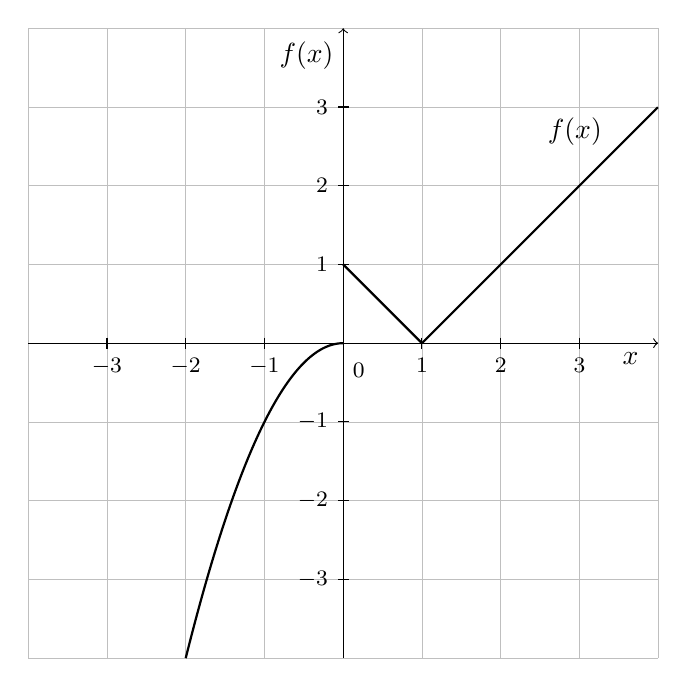
\begin{tikzpicture}
	
	% Gitternetzlinien
	\draw[xstep=1cm, ystep=1cm, very thin, color=lightgray] (-4,4) grid (4,-4);
	% x-Achse
	\draw[->] (-4,0) -- (4,0) node[below,xshift=-1em] {$x$}; 
	%Zahlen auf x-Achse
	\foreach \x in {-3,...,-1}
	\draw[shift={(\x,0)},color=black] (0pt,2pt) -- (0pt,-2pt) node[below] {\footnotesize $\x$};
	\foreach \x in {1,...,3}
	\draw[shift={(\x,0)},color=black] (0pt,2pt) -- (0pt,-2pt) node[below] {\footnotesize $\x$};
	% y-Achse 
	\draw[->] (0,-4) -- (0,4) node[left,yshift=-1em] {$f(x)$};%node[above left]
	%Zahlen auf y-Achse
	\foreach \y in {-1,...,-3}
	\draw[shift={(0,\y)},color=black] (2pt,0pt) -- (-2pt,0pt) node[left] {\footnotesize $\y$};
	\foreach \y in {1,...,3}
	\draw[shift={(0,\y)},color=black] (2pt,0pt) -- (-2pt,0pt) node[left] {\footnotesize $\y$};
	%Ursprung
	\draw[color=black] (0pt,-10pt) node[right] {\footnotesize $0$};
	
	\draw[thick,color=black] plot[samples=200, domain=-2:0] 
	(\x,{-\x*\x});
	
	\draw[thick,color=black] plot[samples=200, domain=0:1] 
	(\x,{-\x+1});
	
	\draw[thick,color=black] plot[samples=200, domain=1:4] 
	(\x,{\x-1}) node[below, xshift=-3em]{$f(x)$};
	
	\end{tikzpicture}\\	
\end{center}
Frage: Welche Stellen muß ich untersuchen?\\
\begin{quote}
	\textbullet \;\; $ |1-x| =     \left\{ \begin{array}{rcl}
	-1+x & \mbox{für} & x\geq 1\\
	1-x & \mbox{für} & x < 1 \\
	
	\end{array}\right. $\\
	\textbullet \;\; $ x_0=0$\\
\end{quote}
Für $ x\neq 1,0 $ ist $ f $ als Komposition stetiger Funktion stetig.\vspace*{2mm}\\
\newpage
\noindent
\textbullet \;\; Bei der Stelle: $ x_0=1 $:
\begin{quote}
	zu zeigen:\\
	\begin{align*}
	&\lim\limits_ {\substack{x \to 1 \\ x>1}} f(x)=	\lim\limits_ {\substack{x \to 1 \\ x>1}}|1-x|=\lim\limits_ {x\to\ 1}(-1+x)=0\\
	&\lim\limits_ {\substack{x \to 1 \\ x<1}} f(x)=	\lim\limits_ {\substack{x \to 1 \\ x<1}}|1-x|=\lim\limits_ {x\to\ 1}1-x=0\\
	&f(1)=|1-1|=0\\
	&\Rightarrow\\
	&\lim\limits_ {\substack{x \to 1 \\ x>1}} f(x)=\lim\limits_ {\substack{x \to 1 \\ x<1}}f(x)=f(x)\\
	&\Rightarrow f\;\; \text{in }\;\;x_0=1\;\;\text{stetig }
	\end{align*}
	
\end{quote}
\textbullet \;\; Bei der Stelle: $ x_0=0 $:
\begin{quote}
	zu zeigen:\\
	\begin{align*}
	&\lim\limits_ {\substack{x \to 0 \\ x>0}}f(x)=\lim\limits_ {\substack{x \to 0 \\ x>0}}1-x=1\\
	&\lim\limits_ {\substack{x \to 0 \\ x<0}}f(x)=\lim\limits_ {\substack{x \to 0 \\ x<0}}-x^2=0\\
	&\Rightarrow\\
	&\lim\limits_ {\substack{x \to 0 \\ x>0}}f(x)\neq\lim\limits_ {\substack{x \to 0 \\ x<0}}f(x)\\
	&\Rightarrow f\;\; \text{nicht in }\;\;x_0=0\;\;\text{stetig }
	\end{align*}
\end{quote}
Fazit:\\
\begin{quote}
	$ f $ ist für $ x\in \mathbb{R}\backslash\{0\} $ stetig.\\
\end{quote}
\subsubsection{Aufgabe 2 zu Rechenregeln von stetigen Funktionen}
\href{https://youtu.be/hae5ZE-L7QU}{Video 09}\\
Wähle $ \alpha ,\beta \in\mathbb{R} $ , s.d. die folgende Funktion stetig ist:\\
\begin{align*}
f(x) =     \left\{ \begin{array}{rcr}
\mathrm{e}^x & \mbox{für} & x\geq 0\\
\alpha \cos(x)+\beta \sin(x) & \mbox{für} & -\frac{\pi}{2}\leq x < 0 \\
2+(x+\frac{\pi}{2})^2 & \mbox{für} & x< -\frac{\pi}{2}\\
\end{array}\right.
\end{align*}
In den Bereichen:\\
\begin{align*}
&x\in \;\; ]0,\infty[\\
&x\in \;\;]-\frac{\pi}{2},0[ \\
&x\in \;\;]-\infty,-\frac{\pi}{2}[\\
\end{align*}
ist $ f $ als Komposition stetiger Abb. stetig.\\
\newpage
\noindent
\textbullet\;\; Bei der Stelle $ x_0=0 $:\\
\begin{quote}
	zu zeigen:\\
	\begin{align*}
	&\lim\limits_ {\substack{x \to 0 \\ x>0}}f(x)=\lim\limits_ {\substack{x \to 0 \\ x<0}}f(x)=f(0)\\
	&\lim\limits_ {\substack{x \to 0 \\ x>0}}f(x)=\lim\limits_ {x\to 0}\mathrm{e}^x=1\\
	&\lim\limits_ {\substack{x \to 0 \\ x<0}}f(x)=\lim\limits_ {x\to 0}(\alpha \cos(x)+\beta \sin(x))=\alpha\cdot 1+\beta \cdot0=f(0)=\mathrm{e}^0=1\\
	&\Rightarrow \text{für }\;\;\alpha=1\;\text{ ist}\;f \;\;\text{in }\;\;x_0=0\;\;\text{stetig }
	\end{align*}
	
\end{quote}
\textbullet\;\; Bei der Stelle $ x_0=-\frac{\pi}{2} $:\\
\begin{quote}
	zu zeigen:
	\begin{align*}
	&\lim\limits_ {\substack{x \to -\frac{\pi}{2}  \\ x<-\frac{\pi}{2}}}f(x)=\lim\limits_ {\substack{x \to -\frac{\pi}{2} \\ x>-\frac{\pi}{2}}}f(x)=f(-\genfrac{}{}{}{2}{\pi}{2 })\\
	&\lim\limits_ {\substack{x \to -\frac{\pi}{2}  \\ x<-\frac{\pi}{2}}}f(x)=\lim\limits_ {x\to -\frac{\pi}{2}}\big(2+(x+\genfrac{}{}{}{2}{\pi}{2})^2\big)=2\\
	&\lim\limits_ {\substack{x \to -\frac{\pi}{2}  \\ x>-\frac{\pi}{2}}}f(x)=\lim\limits_ {x\to -\frac{\pi}{2}}(\alpha \cos(x)+\beta \sin(x)=\alpha\cdot 0+\beta(-1)=-ß\\
	&f(-\genfrac{}{}{}{2}{\pi }{2})=\alpha \cos(-\genfrac{}{}{}{2}{\pi}{2})+\beta \sin(-\genfrac{}{}{}{2}{\pi}{2})=-\beta\\
	&\Rightarrow \text{für }\;\;\beta=-2\;\text{ ist}\;f \;\;\text{in }\;\;x_0=-\frac{\pi}{2}\;\;\text{stetig }
	\end{align*}
\end{quote}
Fazit:\\
Für $ \alpha=1 $ und $ \beta=-2 $ ist $ f $ stetig.\\
\subsection{Epsilon-Delta Definition}
\href{https://youtu.be/4twSaHZ1G3g}{Video 05}\\
Definition (Epsilon-Delta Kriterium):\vspace*{2mm}\\
Die Funktion $ f:\mathbb{D}\subset \mathbb{R}\longmapsto\mathbb{R} $ ist stetig in $ x_0\in \mathbb{D} $, wenn zu jedem $ \varepsilon > 0 $ ein $ \delta>0 $ existiert, so dass für alle $ x\in \mathbb{D} $ mit $ |x-x_0|<\delta $ gilt $ |f(x)-f(x_0)<\varepsilon $.\\
Oder in math. Kurzschreibweise:\\
\begin{align*}
\forall\varepsilon>0\;\exists\delta>0\;\forall x\in \mathbb{D}:(|x-x_0|<\delta\Rightarrow|f(x)-f(x_0|<\varepsilon)
\end{align*}
\begin{center}
	
	
	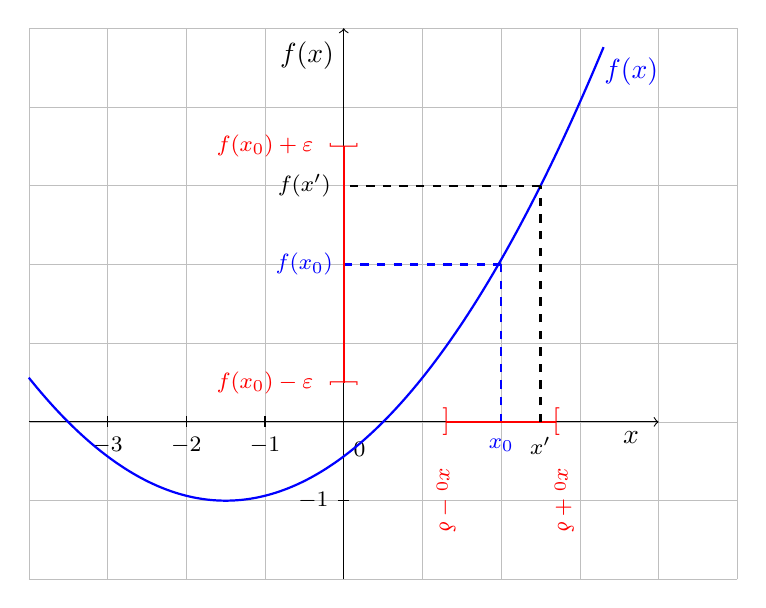
\begin{tikzpicture}
	
	% Gitternetzlinien
	\draw[xstep=1cm, ystep=1cm, very thin, color=lightgray] (-4,5) grid (5,-2);
	% x-Achse
	\draw[->] (-4,0) -- (4,0) node[below,xshift=-1em] {$x$}; 
	%Zahlen auf x-Achse
	\foreach \x in {-3,...,-1}
	\draw[shift={(\x,0)},color=black] (0pt,2pt) -- (0pt,-2pt) node[below] {\footnotesize $\x$};
	%\foreach \x in {1,...,3}
	%\draw[shift={(\x,0)},color=black] (0pt,2pt) -- (0pt,-2pt) node[below] {\footnotesize $\x$};
	% y-Achse 
	\draw[->] (0,-2) -- (0,5) node[left,yshift=-1em] {$f(x)$};%node[above left]
	%Zahlen auf y-Achse
	\foreach \y in {-1,...,-1}
	\draw[shift={(0,\y)},color=black] (2pt,0pt) -- (-2pt,0pt) node[left] {\footnotesize $\y$};
	%foreach \y in {1,...,3}
	%draw[shift={(0,\y)},color=black] (2pt,0pt) -- (-2pt,0pt) node[left] {\footnotesize $\y$};
	%Ursprung
	\draw[color=black] (0pt,-10pt) node[right] {\footnotesize $0$};
	
	
	
	\draw[thick,color=blue] plot[samples=200, domain=-4:3.3] 
	(\x,{0.25*(\x+1.5)^2-1}) node[below, xshift=1em]{$f(x)$};
	\draw[color=blue,dashed,thick] (2,0)--(2,2);
	\draw[color=blue] (2,-0.3) node{\footnotesize $x_0$};
	\draw[color=blue,dashed,thick] (0,2)--(2,2);
	\draw[color=blue] (-0.5,2) node{\footnotesize $f(x_0)$};
	\draw[color=red,thick] (0,0.5)--(0,3.5);
	\draw[color=red,thick] (-1,3.5)node{\footnotesize $f(x_0)+\varepsilon$};
	\draw[color=red,thick] (-1,0.5)node{\footnotesize $f(x_0)-\varepsilon$};
	%\draw[color=red,thick,rotate=90] (0,3)node{\footnotesize $[$};
	\node at (0,3.5) [rotate=90,color=red] {$[$};
	\node at (0,0.5) [rotate=-90,color=red] {$[$};
	%\draw[color=red,thick,dashed] (2.5,0)--(2.5,3);
	%\draw[color=red,thick,dashed] (2.5,3)--(0,3);
	%\draw[color=red,thick,dashed] (0,1)--(1.35,1);
	%\draw[color=red,thick,dashed] (1.35,1)--(1.35,0);
	\draw[color=red,thick] (1.3,0)--(2.7,0);
	\node at (1.3,0) [rotate=0,color=red] {$]$};
	\node at (2.7,0) [rotate=0,color=red] {$[$};
	\node at (2.8,-1) [rotate=-90,color=red] {\footnotesize $x_0+\delta$};
	\node at (1.3,-1) [rotate=-90,color=red] {\footnotesize $x_0-\delta$};
	\draw[color=black] (2.5,-0.3) node{\footnotesize $x^\prime$};
	\draw[color=black,thick,dashed] (2.5,0)--(2.5,3);
	\draw[color=black,thick,dashed] (2.5,3)--(0,3);
	\draw[color=black] (-0.5,3) node{\footnotesize $f(x^\prime )$};
	\end{tikzpicture}\\
	Hier gilt:\\
	\begin{align*}
	\forall\varepsilon>0\;\exists\;\delta>0\;\forall x^\prime \in \mathbb{D} :(|x^\prime -x_0|<\delta \Rightarrow
	|f(x^ \prime)-f(x_0)|<\varepsilon) \\
	\end{align*}
\end{center}
\begin{center}
	
	
	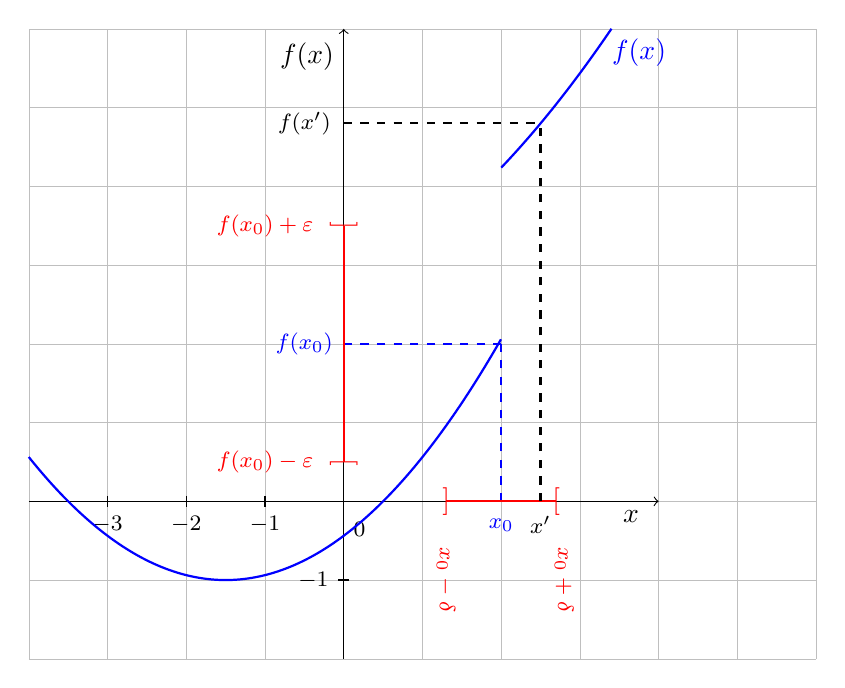
\begin{tikzpicture}
	
	% Gitternetzlinien
	\draw[xstep=1cm, ystep=1cm, very thin, color=lightgray] (-4,6) grid (6,-2);
	% x-Achse
	\draw[->] (-4,0) -- (4,0) node[below,xshift=-1em] {$x$}; 
	%Zahlen auf x-Achse
	\foreach \x in {-3,...,-1}
	\draw[shift={(\x,0)},color=black] (0pt,2pt) -- (0pt,-2pt) node[below] {\footnotesize $\x$};
	%\foreach \x in {1,...,3}
	%\draw[shift={(\x,0)},color=black] (0pt,2pt) -- (0pt,-2pt) node[below] {\footnotesize $\x$};
	% y-Achse 
	\draw[->] (0,-2) -- (0,6) node[left,yshift=-1em] {$f(x)$};%node[above left]
	%Zahlen auf y-Achse
	\foreach \y in {-1,...,-1}
	\draw[shift={(0,\y)},color=black] (2pt,0pt) -- (-2pt,0pt) node[left] {\footnotesize $\y$};
	%foreach \y in {1,...,3}
	%draw[shift={(0,\y)},color=black] (2pt,0pt) -- (-2pt,0pt) node[left] {\footnotesize $\y$};
	%Ursprung
	\draw[color=black] (0pt,-10pt) node[right] {\footnotesize $0$};
	\draw[thick,color=blue] plot[samples=200, domain=-4:2] 
	(\x,{0.25*(\x+1.5)^2-1});
	
	
	\draw[thick,color=blue] plot[samples=200, domain=2:3.4] 
	(\x,{0.15*(\x+1.5)^2+2.4}) node[below, xshift=1em]{$f(x)$};
	\draw[color=blue,dashed,thick] (2,0)--(2,2);
	\draw[color=blue] (2,-0.3) node{\footnotesize $x_0$};
	\draw[color=blue,dashed,thick] (0,2)--(2,2);
	\draw[color=blue] (-0.5,2) node{\footnotesize $f(x_0)$};
	\draw[color=red,thick] (0,0.5)--(0,3.5);
	\draw[color=red,thick] (-1,3.5)node{\footnotesize $f(x_0)+\varepsilon$};
	\draw[color=red,thick] (-1,0.5)node{\footnotesize $f(x_0)-\varepsilon$};
	%\draw[color=red,thick,rotate=90] (0,3)node{\footnotesize $[$};
	\node at (0,3.5) [rotate=90,color=red] {$[$};
	\node at (0,0.5) [rotate=-90,color=red] {$[$};
	%\draw[color=red,thick,dashed] (1.3,0)--(1.3,0.8);
	%\draw[color=red,thick,dashed] (2.5,3)--(0,3);
	%\draw[color=red,thick,dashed] (0,1)--(1.35,1);
	%\draw[color=red,thick,dashed] (1.35,1)--(1.35,0);
	\draw[color=red,thick] (1.3,0)--(2.7,0);
	\node at (1.3,0) [rotate=0,color=red] {$]$};
	\node at (2.7,0) [rotate=0,color=red] {$[$};
	\node at (2.8,-1) [rotate=-90,color=red] {\footnotesize $x_0+\delta$};
	\node at (1.3,-1) [rotate=-90,color=red] {\footnotesize $x_0-\delta$};
	\draw[color=black] (2.5,-0.3) node{\footnotesize $x^\prime$};
	\draw[color=black,thick,dashed] (2.5,0)--(2.5,4.8);
	\draw[color=black,thick,dashed] (0,4.8)--(2.5,4.8);
	\draw[color=black] (-0.5,4.8) node{\footnotesize $f(x^\prime )$};
	\end{tikzpicture}\\
	Es gilt nicht mehr:\\
	\begin{align*}
	\forall\varepsilon>0\;\exists\;\delta>0\;\forall x^\prime \in \mathbb{D} :(|x^\prime -x_0|<\delta \Rightarrow
	|f(x^ \prime)-f(x_0)|<\varepsilon) \\
	\end{align*}
	
\end{center}
Bemerkung:\\
Eine Funktion $ f $ heißt stetig in $ \mathbb{D} $, wenn $ f $ stetig in allen $ x_0\in \mathbb{D} $ ist.\\
\subsubsection{Beispiel Epsilon-Delta Definition}
\href{https://youtu.be/1SoRceatdgo}{Video 06}\\
Zeige, dass $ f:\mathbb{R}\longmapsto\mathbb{R} $ mit $ f(x)=x^2 $ in $ x_0=0 $ stetig ist.\vspace*{2mm}\\
Zu zeigen:\\
\begin{align*}
\forall\;\varepsilon>0\;\exists\;\delta >0\;\forall x\in \mathbb{R}:(|x-x_0|<\varepsilon\Rightarrow|f(x)-f(x_0)|<\delta)
\end{align*}
Sei $ \varepsilon>0 $ beliebig:\\
Es gilt für $ x_0=0 $ :\\
\begin{align}
|x-x_0|<\delta \nonumber\\
|x|<\delta 
\end{align}
Und es gilt für $ f(x)=x^2 $ und $ f(x_0)=x_0^2 $\\
\begin{align}
|f(x)-f(x_0)|<\varepsilon \nonumber\\
|x^2-x_0^2|=|x^2|<\varepsilon
\end{align}
In Gleichung (VI.2) Gleichung (VI.1) einsetzen:\\
\begin{align*}
|\delta^2|<\varepsilon\\
\delta<\sqrt{\varepsilon}\\
\end{align*}
Wähle: $ 0<\delta<\sqrt{\varepsilon} $\\
Beweis mit: $ \varepsilon>0 $ mit $ \delta=\sqrt{\varepsilon}\;\;\forall x\in \mathbb{R} $ mit $ |x|<\delta $\\
\begin{align*}
|f(x)-f(x_0)|&=|x^2|\\
&<|\delta^2| \;\;\text{mit } \delta=\sqrt{\varepsilon}\\
&<|\sqrt{\varepsilon}^2|\\|f(x)-f(x_0)|&<\varepsilon_{_{\Square}}
\end{align*}
\subsubsection{Aufgabe Epsilon-Delta Definition}
\href{https://youtu.be/Qnf4afRSK38}{Video 07}\\
Zeige, dass $ f:\mathbb{R}\longmapsto\mathbb{R} $ mit $ f(x)=\frac{x-1}{x^2+1} $ in $ x_0=-1 $ stetig ist.\vspace*{2mm}\\
Zu zeigen:\\
\begin{align*}
\forall\;\varepsilon>0\;\exists\;\delta >0\;\forall x\in \mathbb{R}:(|x-x_0|<\varepsilon\Rightarrow|f(x)-f(x_0)|<\delta)
\end{align*}
Es gilt für $ x_0=-1 $ :\\
\begin{align*}
|x-x_0&|<\delta\\
|x-(-1)|&<\delta\\
|x+1|&<\delta
\end{align*}
\newpage
\noindent
Und es gilt:\\
\begin{align*}
|f(x)-f(x_0)&<\varepsilon\\
\bigg|\frac{x-1}{x^2+1}-\frac{x_0-1}{x_0^2+1}\bigg|&<\varepsilon\\
\bigg|\frac{x-1}{x^2+1}-\frac{-2}{2}\bigg|&<\varepsilon\\
\bigg|\frac{x-1}{x^2+1}+1\bigg|&<\varepsilon\\
\bigg|\frac{x-1+x^2+1}{x^2+1}\bigg|&<\varepsilon\\
\bigg|\frac{x^2+x}{x^2+1}\bigg|&<\varepsilon\\
\bigg|\frac{x(x+1)}{x^2+1}\bigg|&<\varepsilon\\
\bigg|\frac{x}{x^2+1}\bigg|\bigg|x+1\bigg|&<\varepsilon
\end{align*}
Behauptung:\\
\begin{align*}
\bigg|\frac{x}{x^2+1}\bigg|<1\;\;\forall x\in\mathbb{R}
\end{align*}
Beweis:\\
\begin{align*}
&\bigg|\frac{x}{x^2+1}\bigg|<1\\
&\Leftrightarrow |x|<|x^2+1|\;\;\forall x\in\mathbb{R}_{_{\;\;\Square}}
\end{align*}
Zur Stetigkeit:\\
Sei $ \varepsilon>0 $ beliebig und wähle $ \delta=\varepsilon $ dann gilt für:\\
\begin{align*}
|x-x_0|=|x+1|<\delta=\varepsilon
\end{align*}
dass
\begin{align*}
|f(x)-f(x_0)|=\underbrace {\bigg|\frac{x}{x^2+1}\bigg|}_{<1}\underbrace {\bigg|x+1\bigg|}_{<\delta=\varepsilon}<\varepsilon_{\;\;_{\Square}}
\end{align*}
\subsection{Zwischenwertsatz}
\href{https://youtu.be/qJcBXQWDClk}{Video 10}\\
\begin{center}
	\fbox{\parbox  {84mm} {
			Sei $ I\subseteq \mathbb{R} $ ein Intervall und $ f:I\longmapsto\mathbb{R} $ stetig.\\
			Seien $ a,b \in I $ und $ y_0 $ zwischen $ f(a) $ und $ f(b) $.\\
			Dann existiert ein $ x_0 \in [ a,b]   $ mit $ f(x_0)=y_0 $}}
\end{center}
\begin{center}
	
	
	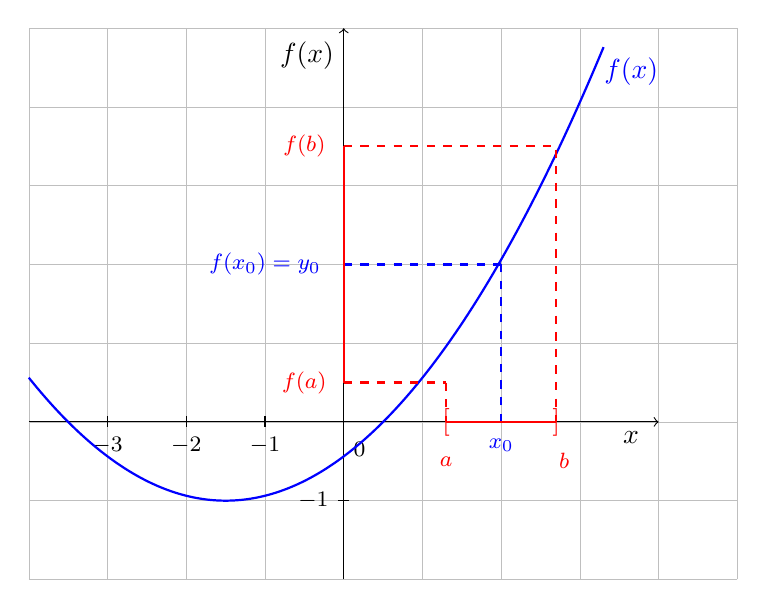
\begin{tikzpicture}
	
	% Gitternetzlinien
	\draw[xstep=1cm, ystep=1cm, very thin, color=lightgray] (-4,5) grid (5,-2);
	% x-Achse
	\draw[->] (-4,0) -- (4,0) node[below,xshift=-1em] {$x$}; 
	%Zahlen auf x-Achse
	\foreach \x in {-3,...,-1}
	\draw[shift={(\x,0)},color=black] (0pt,2pt) -- (0pt,-2pt) node[below] {\footnotesize $\x$};
	%\foreach \x in {1,...,3}
	%\draw[shift={(\x,0)},color=black] (0pt,2pt) -- (0pt,-2pt) node[below] {\footnotesize $\x$};
	% y-Achse 
	\draw[->] (0,-2) -- (0,5) node[left,yshift=-1em] {$f(x)$};%node[above left]
	%Zahlen auf y-Achse
	\foreach \y in {-1,...,-1}
	\draw[shift={(0,\y)},color=black] (2pt,0pt) -- (-2pt,0pt) node[left] {\footnotesize $\y$};
	%foreach \y in {1,...,3}
	%draw[shift={(0,\y)},color=black] (2pt,0pt) -- (-2pt,0pt) node[left] {\footnotesize $\y$};
	%Ursprung
	\draw[color=black] (0pt,-10pt) node[right] {\footnotesize $0$};
	
	
	
	\draw[thick,color=blue] plot[samples=200, domain=-4:3.3] 
	(\x,{0.25*(\x+1.5)^2-1}) node[below, xshift=1em]{$f(x)$};
	\draw[color=blue,dashed,thick] (2,0)--(2,2);
	\draw[color=blue] (2,-0.3) node{\footnotesize $x_0$};
	\draw[color=blue,dashed,thick] (0,2)--(2,2);
	\draw[color=blue] (-1,2) node{\footnotesize $f(x_0)=y_0$};
	\draw[color=red,thick] (0,0.5)--(0,3.5);
	\draw[color=red,thick] (-0.5,3.5)node{\footnotesize $f(b)$};
	\draw[color=red,thick] (-0.5,0.5)node{\footnotesize $f(a)$};
	%\draw[color=red,thick,rotate=90] (0,3)node{\footnotesize $[$};
	
	\draw[color=red,thick,dashed] (0,0.5)--(1.3,0.5);
	\draw[color=red,thick,dashed] (1.3,0.5)--(1.3,0);
	\draw[color=red,thick,dashed] (0,3.5)--(2.7,3.5)--(2.7,0);
	%\draw[color=red,thick,dashed] (1.35,1)--(1.35,0);
	\draw[color=red,thick] (1.3,0)--(2.7,0);
	\node at (1.3,0) [rotate=180,color=red] {$]$};
	\node at (2.7,0) [rotate=180,color=red] {$[$};
	\node at (2.8,-0.5) [rotate=0,color=red] {\footnotesize $b$};
	\node at (1.3,-0.5) [rotate=0,color=red] {\footnotesize $a$};
	
	\end{tikzpicture}\\
	
\end{center}
Liegt ein Wert zwischen $ f(a) $ und $ f(b) $, dann findet man einen Wert der zwischen $ a $ und $ b $ liegt. Natürlich nur bei einer stetigen Abbildung.\\
Den Zwischenwertsatz (ZWS) benötigt man zur Berechnung von Nullstellen einer Funktion, wenn diese Nullstelle nicht algebraisch berechenbar ist.\vspace*{2mm}\\
Beispiel:\\
Betrachte: $ f:\mathbb{R}\longmapsto \mathbb{R} $ mit $ f(x)=x-1 $\\
Zeige, dass $ f(x) $ eine Nullstelle hat.\\
\begin{center}
	
	
	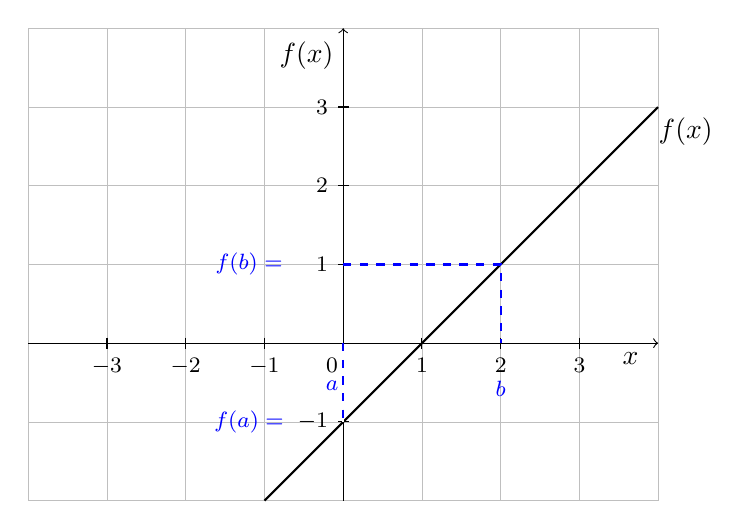
\begin{tikzpicture}
	
	% Gitternetzlinien
	\draw[xstep=1cm, ystep=1cm, very thin, color=lightgray] (-4,4) grid (4,-2);
	% x-Achse
	\draw[->] (-4,0) -- (4,0) node[below,xshift=-1em] {$x$}; 
	%Zahlen auf x-Achse
	\foreach \x in {-3,...,-1}
	\draw[shift={(\x,0)},color=black] (0pt,2pt) -- (0pt,-2pt) node[below] {\footnotesize $\x$};
	\foreach \x in {1,...,3}
	\draw[shift={(\x,0)},color=black] (0pt,2pt) -- (0pt,-2pt) node[below] {\footnotesize $\x$};
	% y-Achse 
	\draw[->] (0,-2) -- (0,4) node[left,yshift=-1em] {$f(x)$};%node[above left]
	%Zahlen auf y-Achse
	\foreach \y in {-1,...,-1}
	\draw[shift={(0,\y)},color=black] (2pt,0pt) -- (-2pt,0pt) node[left] {\footnotesize $\y$};
	\foreach \y in {1,...,3}
	\draw[shift={(0,\y)},color=black] (2pt,0pt) -- (-2pt,0pt) node[left] {\footnotesize $\y$};
	%Ursprung
	\draw[color=blue] (-4pt,-10pt) node[below] {\footnotesize $a$};
	\draw[color=blue] (2,-10pt) node[below] {\footnotesize $b$};
	\draw[color=black] (-4pt,-2pt) node[below] {\footnotesize $0$};
	\draw[color=blue] (-34pt,1) node {\footnotesize $f(b)=$};
	\draw[thick,color=black] plot[samples=200, domain=-1:4] 
	(\x,{\x-1}) node[below, xshift=1em]{$f(x)$};
	\draw[color=blue,thick, dashed] (0,1)--(2,1)--(2,0);
	\draw[color=white,thick] (0,0)--(0,-1);
	\draw[color=blue,thick, dashed] (0,0)--(0,-1);
	\draw[color=blue] (-34pt,-1) node {\footnotesize $f(a)=$};
	\end{tikzpicture}\\
\end{center}
(i)
\begin{quote}
	Offensichtlich ist $ f $ stetig.
\end{quote}
(ii)
\begin{quote}
	Betrachte: $ f(2)=2-1+1 >0$ 
\end{quote}
(ii)
\begin{quote}
	Betrachte: $ f(0)=0-1 <0$ 
\end{quote}
Nach dem ZWS gilt:\\
\begin{align*}
-1=f(0)<y_0=0<f(2)=1
\end{align*}
Es existiert ein $ x_0\in [0,2] $ mit $ f(x_0)=y_0=0 $, d.h. $ x_0 $ ist eine Nullstelle von $ f $.\\
Die Nullstelle algebraisch gerechnet ist $ x_0=1 $\\
\subsubsection{Aufgabe zum Zwischenwertsatz}
\href{https://youtu.be/hsNWvy0z_VE}{Video 11}\\
Zeige, dass die Gleichung $ \sin(x)=1-\frac{\sin(x)}{\cos(x)} $ eine Lösung im Intervall $ [-\frac{\pi}{4},\frac{\pi}{4}] $ hat.\vspace*{2mm}\\
Betrachte mit der Hilfsfunktion $ h(x) $:\\
\begin{align*}
h(x)=1-\frac{\sin(x)}{\cos(x)}-\sin(x)\;\;\text{wenn }\;\;h(x)=0
\end{align*}
Dann gilt:
\begin{align*}
\sin(x)=1-\frac{\sin(x)}{\cos(x)}
\end{align*}
D.h., wir suchen $ x_0 \in [-\frac{\pi}{4},\frac{\pi}{4}]$  mit $ h(x) =0.$\\
(i)
\begin{quote}
	
	\begin{align*}
	h(- \genfrac{}{}{}{2}{\pi }{4})=1-\frac{\sin(-\genfrac{}{}{}{2}{\pi}{4 })}{\cos(-\genfrac{}{}{}{2}{\pi }{4 })}-\sin(-\genfrac{}{}{}{2}{\pi }{4 })=1-\frac{-\genfrac{}{}{}{2}{1}{\sqrt{2}}}{\genfrac{}{}{}{2}{1 }{\sqrt{2} }}-(-\genfrac{}{}{}{2}{1 }{\sqrt{2} })=2+\frac{1}{\sqrt{2}}>0
	\end{align*}
\end{quote}
(ii)
\begin{quote}
	
	\begin{align*}
	h( \genfrac{}{}{}{2}{\pi }{4})=1-\frac{\sin(\genfrac{}{}{}{2}{\pi}{4 })}{\cos(\genfrac{}{}{}{2}{\pi }{4 })}-\sin(\genfrac{}{}{}{2}{\pi }{4 })=1-\frac{\genfrac{}{}{}{2}{1}{\sqrt{2}}}{\genfrac{}{}{}{2}{1 }{\sqrt{2} }}-\frac{1}{\sqrt{2}}=-\frac{1}{\sqrt{2}}<0
	\end{align*}
\end{quote}


Skizze von Cosinus und Sinus:\\
\begin{center}
	
	
	\begin{tikzpicture}[scale=2]
	
	% Gitternetzlinien
	\draw[xstep=1cm, ystep=1cm, very thin, color=lightgray] (-3.5,2) grid (3.5,-2);
	% x-Achse
	\draw[->] (-3.5,0) -- (3.5,0) node[below,xshift=-1em] {$x$}; 
	%Zahlen auf x-Achse
	\foreach \x in {-2,...,-1}
	\draw[shift={(\x,0)},color=black] (0pt,2pt) -- (0pt,-2pt) node[below] {\footnotesize $\x$};
	\foreach \x in {1,...,2}
	\draw[shift={(\x,0)},color=black] (0pt,2pt) -- (0pt,-2pt) node[below] {\footnotesize $\x$};
	% y-Achse 
	\draw[->] (0,-2) -- (0,2) node[left,yshift=-1em] {$f(x)$};%node[above left]
	%Zahlen auf y-Achse
	\foreach \y in {-1,...,-1}
	\draw[shift={(0,\y)},color=black] (2pt,0pt) -- (-2pt,0pt) node[left] {\footnotesize $\y$};
	\foreach \y in {1,...,1}
	\draw[shift={(0,\y)},color=black] (2pt,0pt) -- (-2pt,0pt) node[left] {\footnotesize $\y$};
	%Ursprung
	\draw[color=black] (0pt,-10pt) node[right] {\footnotesize $0$};
	
	\draw[thick,color=blue] plot[samples=200, domain=-3.5:3.5] 
	(\x,{sin(\x r)}) node[xshift=-1em,yshift=4.5em]{$\sin(x)$};
	\draw[thick,color=red] plot[samples=200, domain=-3.5:3.5] 
	(\x,{cos(\x r)}) node[xshift=1em,yshift=1.5em]{$\cos(x)$};
	\draw[color=green] (-3.14/4,-1.2) node {\footnotesize $-\genfrac{}{}{}{2}{\pi }{4 }$};
	\draw[color=green] (3.14/4,-1.2) node {\footnotesize $\genfrac{}{}{}{2}{\pi }{4 }$};
	\draw[color=green] (3.14/4,1)--(3.14/4,-1);
	\draw[color=green] (-3.14/4,1)--(-3.14/4,-1);
	\end{tikzpicture}\\
	\begin{align*}
	&\cos(\genfrac{}{}{}{2}{\pi }{4})=\sin(\genfrac{}{}{}{2}{\pi }{4})=\frac{1}{\sqrt{2}}\\
	&\cos(-\genfrac{}{}{}{2}{\pi }{4})=\frac{1}{\sqrt{2}}\\
	&\sin(-\genfrac{}{}{}{2}{\pi }{4})=-\frac{1}{\sqrt{2}}\\
	\end{align*}
\end{center}
(iii)
\begin{quote}
	$ h(x) $ ist als Komposition stetiger Funktionen stetig auf $ [-\frac{\pi}{4},\frac{\pi}{4}] $\\
\end{quote}
Nach dem ZWS gilt im Intervall $x_0\in [-\frac{\pi}{4},\frac{\pi}{4}]  $ mit $ h(x_0)=y_0=0 $:\\
\begin{align*}
h(-\genfrac{}{}{}{2}{\pi }{4})<y_0=0<h(\genfrac{}{}{}{2}{\pi }{4})\\
\end{align*}
Dann ist $ x_0 $ auch eine Lösung der Ausgangsgleichung.\\
\subsection{Extrema von Funktionen}
\href{https://youtu.be/la8s-zLqf5w}{Video 12}\\
\underline{Definition(Maximum, Minimum):}\vspace*{2mm}\\
(i) $ f $ nimmt in $ x_0 $ sein globales Maximum $ y_0 $ an, wenn gilt:\\
\begin{align*}
f(x)=y_0\geq f(x)\;\;\text{für alle  } \;\;x\in\mathbb{D}_f
\end{align*}
(ii) $ f $ nimmt in $ x_0 $ sein lokales Minimum $ y_0 $ an, wenn es:\\
\begin{align*}
\varepsilon>0 \;\;\text{gibt mit }\;\;f(x_0)\geq f(x)\;\;\text{für alle }\;\;x\in\mathbb{D}_f\;\;\text{mit }\;\;|x-x_0|<\varepsilon
\end{align*}
Beispiel:\\
\begin{center}
	Globales Maximum\vspace*{2mm}\\	
	
	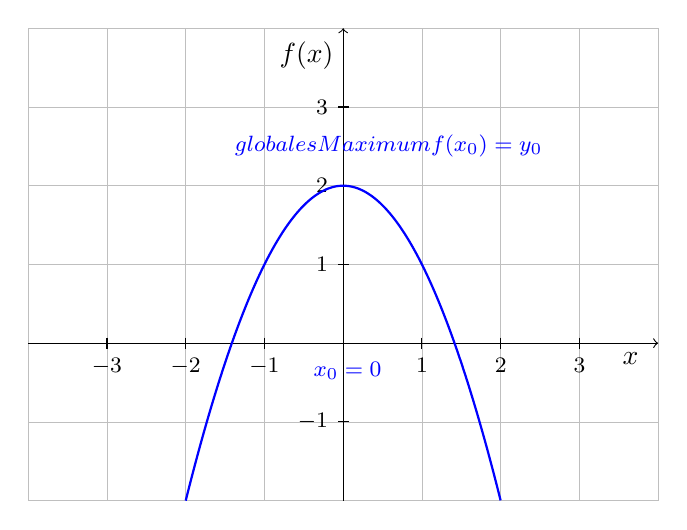
\begin{tikzpicture}
	
	% Gitternetzlinien
	\draw[xstep=1cm, ystep=1cm, very thin, color=lightgray] (-4,4) grid (4,-2);
	% x-Achse
	\draw[->] (-4,0) -- (4,0) node[below,xshift=-1em] {$x$}; 
	%Zahlen auf x-Achse
	\foreach \x in {-3,...,-1}
	\draw[shift={(\x,0)},color=black] (0pt,2pt) -- (0pt,-2pt) node[below] {\footnotesize $\x$};
	\foreach \x in {1,...,3}
	\draw[shift={(\x,0)},color=black] (0pt,2pt) -- (0pt,-2pt) node[below] {\footnotesize $\x$};
	% y-Achse 
	\draw[->] (0,-2) -- (0,4) node[left,yshift=-1em] {$f(x)$};%node[above left]
	%Zahlen auf y-Achse
	\foreach \y in {-1,...,-1}
	\draw[shift={(0,\y)},color=black] (2pt,0pt) -- (-2pt,0pt) node[left] {\footnotesize $\y$};
	\foreach \y in {1,...,3}
	\draw[shift={(0,\y)},color=black] (2pt,0pt) -- (-2pt,0pt) node[left] {\footnotesize $\y$};
	%Ursprung
	%\draw[color=black] (0pt,-10pt) node[right] {\footnotesize $0$};
	
	\draw[thick,color=blue] plot[samples=200, domain=-2:2] 
	(\x,{-\x*\x +2});
	\draw[color=blue] (-1.5,2.5) node[right] {\footnotesize $globales Maximum f(x_0)=y_0$};
	\draw[color=blue] (-0.5,-10pt) node[right] {\footnotesize $x_0=0$};
	
	
	
	
	\end{tikzpicture}\\
\end{center}

\begin{center}
	Lokales Maximum\vspace*{2mm}\\	
	
	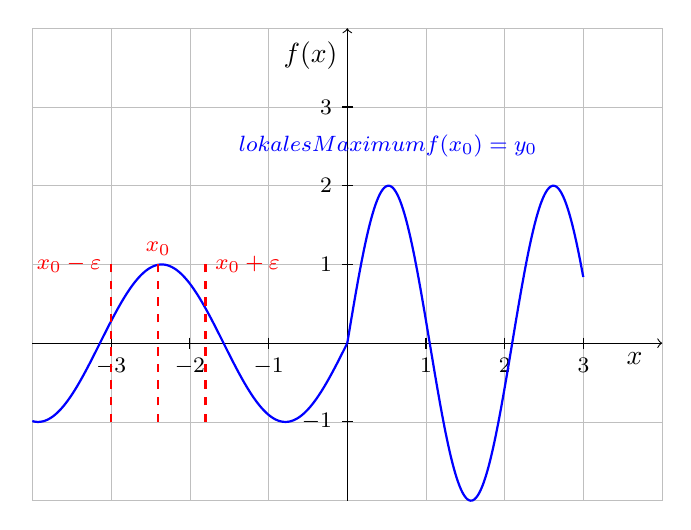
\begin{tikzpicture}
	
	% Gitternetzlinien
	\draw[xstep=1cm, ystep=1cm, very thin, color=lightgray] (-4,4) grid (4,-2);
	% x-Achse
	\draw[->] (-4,0) -- (4,0) node[below,xshift=-1em] {$x$}; 
	%Zahlen auf x-Achse
	\foreach \x in {-3,...,-1}
	\draw[shift={(\x,0)},color=black] (0pt,2pt) -- (0pt,-2pt) node[below] {\footnotesize $\x$};
	\foreach \x in {1,...,3}
	\draw[shift={(\x,0)},color=black] (0pt,2pt) -- (0pt,-2pt) node[below] {\footnotesize $\x$};
	% y-Achse 
	\draw[->] (0,-2) -- (0,4) node[left,yshift=-1em] {$f(x)$};%node[above left]
	%Zahlen auf y-Achse
	\foreach \y in {-1,...,-1}
	\draw[shift={(0,\y)},color=black] (2pt,0pt) -- (-2pt,0pt) node[left] {\footnotesize $\y$};
	\foreach \y in {1,...,3}
	\draw[shift={(0,\y)},color=black] (2pt,0pt) -- (-2pt,0pt) node[left] {\footnotesize $\y$};
	%Ursprung
	%\draw[color=black] (0pt,-10pt) node[right] {\footnotesize $0$};
	
	\draw[thick,color=blue] plot[samples=200, domain=-4:0] 
	(\x,{sin(2*\x r)});
	\draw[thick,color=blue] plot[samples=200, domain=0:3] 
	(\x,{2*sin(3*\x r)});
	\draw[color=blue] (-1.5,2.5) node[right] {\footnotesize $lokales Maximum f(x_0)=y_0$};
	\draw[color=red] (-3,1) node[left] {\footnotesize $x_0-\varepsilon$};
	\draw[color=red] (-1.8,1) node[right] {\footnotesize $x_0+\varepsilon$};
	\draw[color=red,thick,dashed] (-3,-1)--(-3,1) ;
	\draw[color=red,thick,dashed] (-1.8,-1)--(-1.8,1) ;
	\draw[color=red,thick,dashed] (-2.4,-1)--(-2.4,1) ;
	\draw[color=red] (-2.4,1.2) node {\footnotesize $x_0$};
	\end{tikzpicture}\\
\end{center}
Analog definiert man globales und lokales Minimum.\\
\begin{center}
	
	
	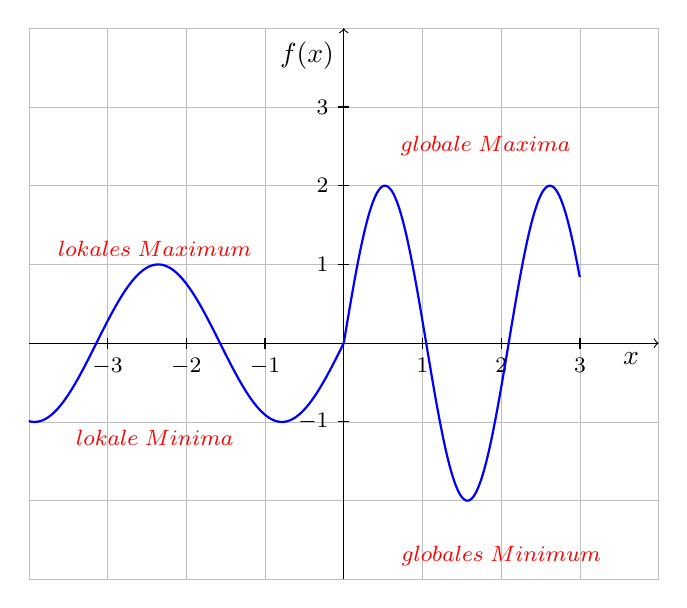
\begin{tikzpicture}
	
	% Gitternetzlinien
	\draw[xstep=1cm, ystep=1cm, very thin, color=lightgray] (-4,4) grid (4,-3);
	% x-Achse
	\draw[->] (-4,0) -- (4,0) node[below,xshift=-1em] {$x$}; 
	%Zahlen auf x-Achse
	\foreach \x in {-3,...,-1}
	\draw[shift={(\x,0)},color=black] (0pt,2pt) -- (0pt,-2pt) node[below] {\footnotesize $\x$};
	\foreach \x in {1,...,3}
	\draw[shift={(\x,0)},color=black] (0pt,2pt) -- (0pt,-2pt) node[below] {\footnotesize $\x$};
	% y-Achse 
	\draw[->] (0,-3) -- (0,4) node[left,yshift=-1em] {$f(x)$};%node[above left]
	%Zahlen auf y-Achse
	\foreach \y in {-1,...,-1}
	\draw[shift={(0,\y)},color=black] (2pt,0pt) -- (-2pt,0pt) node[left] {\footnotesize $\y$};
	\foreach \y in {1,...,3}
	\draw[shift={(0,\y)},color=black] (2pt,0pt) -- (-2pt,0pt) node[left] {\footnotesize $\y$};
	%Ursprung
	%\draw[color=black] (0pt,-10pt) node[right] {\footnotesize $0$};
	
	\draw[thick,color=blue] plot[samples=200, domain=-4:0] 
	(\x,{sin(2*\x r)});
	\draw[thick,color=blue] plot[samples=200, domain=0:3] 
	(\x,{2*sin(3*\x r)});
	\draw[color=red] (-2.4,-1.2) node {\footnotesize $lokale \; Minima$};
	\draw[color=red] (-2.4,1.2) node {\footnotesize $lokales\; Maximum$};
	\draw[color=red] (1.8,2.5) node {\footnotesize $globale\; Maxima$};
	\draw[color=red] (2,-2.7) node {\footnotesize $globales\; Minimum$};
	\end{tikzpicture}\\
\end{center}
\begin{center}
	
	kein globales Maximum\\
	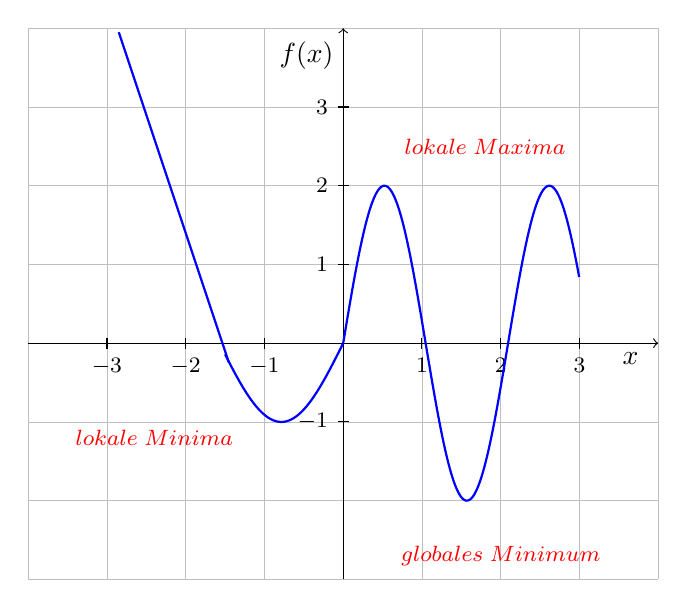
\begin{tikzpicture}
	
	% Gitternetzlinien
	\draw[xstep=1cm, ystep=1cm, very thin, color=lightgray] (-4,4) grid (4,-3);
	% x-Achse
	\draw[->] (-4,0) -- (4,0) node[below,xshift=-1em] {$x$}; 
	%Zahlen auf x-Achse
	\foreach \x in {-3,...,-1}
	\draw[shift={(\x,0)},color=black] (0pt,2pt) -- (0pt,-2pt) node[below] {\footnotesize $\x$};
	\foreach \x in {1,...,3}
	\draw[shift={(\x,0)},color=black] (0pt,2pt) -- (0pt,-2pt) node[below] {\footnotesize $\x$};
	% y-Achse 
	\draw[->] (0,-3) -- (0,4) node[left,yshift=-1em] {$f(x)$};%node[above left]
	%Zahlen auf y-Achse
	\foreach \y in {-1,...,-1}
	\draw[shift={(0,\y)},color=black] (2pt,0pt) -- (-2pt,0pt) node[left] {\footnotesize $\y$};
	\foreach \y in {1,...,3}
	\draw[shift={(0,\y)},color=black] (2pt,0pt) -- (-2pt,0pt) node[left] {\footnotesize $\y$};
	%Ursprung
	%\draw[color=black] (0pt,-10pt) node[right] {\footnotesize $0$};
	\draw[thick,color=blue] plot[samples=200, domain=-2.85:-1.45] 
	(\x,{-3*\x -4.6)});
	\draw[thick,color=blue] plot[samples=200, domain=-1.5:0] 
	(\x,{sin(2*\x r)});
	\draw[thick,color=blue] plot[samples=200, domain=0:3] 
	(\x,{2*sin(3*\x r)});
	\draw[color=red] (-2.4,-1.2) node {\footnotesize $lokale \; Minima$};
	%\draw[color=red] (-2.4,1.2) node {\footnotesize $lokales\; Maximum$};
	\draw[color=red] (1.8,2.5) node {\footnotesize $lokale\; Maxima$};
	\draw[color=red] (2,-2.7) node {\footnotesize $globales\; Minimum$};
	\end{tikzpicture}\\
\end{center}
\begin{center}
	
	kein globales Maximum und Minimum\\
	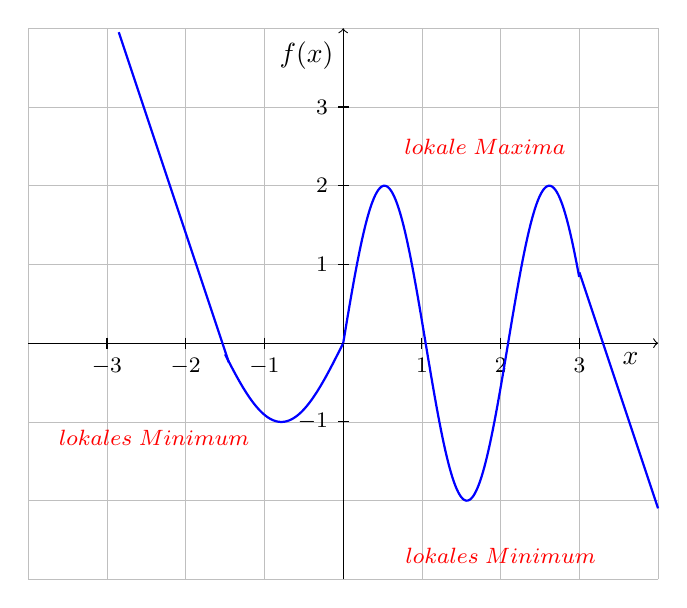
\begin{tikzpicture}
	
	% Gitternetzlinien
	\draw[xstep=1cm, ystep=1cm, very thin, color=lightgray] (-4,4) grid (4,-3);
	% x-Achse
	\draw[->] (-4,0) -- (4,0) node[below,xshift=-1em] {$x$}; 
	%Zahlen auf x-Achse
	\foreach \x in {-3,...,-1}
	\draw[shift={(\x,0)},color=black] (0pt,2pt) -- (0pt,-2pt) node[below] {\footnotesize $\x$};
	\foreach \x in {1,...,3}
	\draw[shift={(\x,0)},color=black] (0pt,2pt) -- (0pt,-2pt) node[below] {\footnotesize $\x$};
	% y-Achse 
	\draw[->] (0,-3) -- (0,4) node[left,yshift=-1em] {$f(x)$};%node[above left]
	%Zahlen auf y-Achse
	\foreach \y in {-1,...,-1}
	\draw[shift={(0,\y)},color=black] (2pt,0pt) -- (-2pt,0pt) node[left] {\footnotesize $\y$};
	\foreach \y in {1,...,3}
	\draw[shift={(0,\y)},color=black] (2pt,0pt) -- (-2pt,0pt) node[left] {\footnotesize $\y$};
	%Ursprung
	%\draw[color=black] (0pt,-10pt) node[right] {\footnotesize $0$};
	\draw[thick,color=blue] plot[samples=200, domain=-2.85:-1.45] 
	(\x,{-3*\x -4.6)});
	\draw[thick,color=blue] plot[samples=200, domain=-1.5:0] 
	(\x,{sin(2*\x r)});
	\draw[thick,color=blue] plot[samples=200, domain=0:3] 
	(\x,{2*sin(3*\x r)});
	\draw[thick,color=blue] plot[samples=200, domain=3:4] 
	(\x,{-3*\x +9.9)});
	\draw[color=red] (-2.4,-1.2) node {\footnotesize $lokales \; Minimum$};
	%\draw[color=red] (-2.4,1.2) node {\footnotesize $lokales\; Maximum$};
	\draw[color=red] (1.8,2.5) node {\footnotesize $lokale\; Maxima$};
	\draw[color=red] (2,-2.7) node {\footnotesize $lokales\; Minimum$};
	\end{tikzpicture}\\
\end{center}
\pagebreak

\begin{center}
	kein globales bzw. lokales Maximum/Minimum\\	
	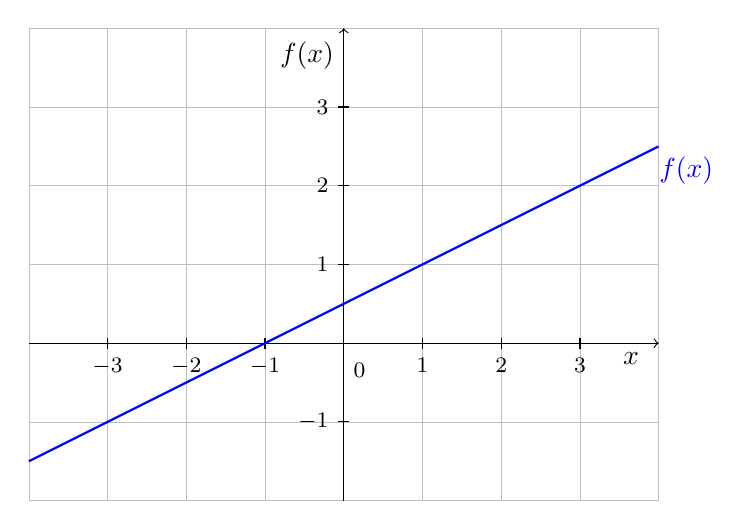
\begin{tikzpicture}
	
	% Gitternetzlinien
	\draw[xstep=1cm, ystep=1cm, very thin, color=lightgray] (-4,4) grid (4,-2);
	% x-Achse
	\draw[->] (-4,0) -- (4,0) node[below,xshift=-1em] {$x$}; 
	%Zahlen auf x-Achse
	\foreach \x in {-3,...,-1}
	\draw[shift={(\x,0)},color=black] (0pt,2pt) -- (0pt,-2pt) node[below] {\footnotesize $\x$};
	\foreach \x in {1,...,3}
	\draw[shift={(\x,0)},color=black] (0pt,2pt) -- (0pt,-2pt) node[below] {\footnotesize $\x$};
	% y-Achse 
	\draw[->] (0,-2) -- (0,4) node[left,yshift=-1em] {$f(x)$};%node[above left]
	%Zahlen auf y-Achse
	\foreach \y in {-1,...,-1}
	\draw[shift={(0,\y)},color=black] (2pt,0pt) -- (-2pt,0pt) node[left] {\footnotesize $\y$};
	\foreach \y in {1,...,3}
	\draw[shift={(0,\y)},color=black] (2pt,0pt) -- (-2pt,0pt) node[left] {\footnotesize $\y$};
	%Ursprung
	\draw[color=black] (0pt,-10pt) node[right] {\footnotesize $0$};
	
	%\draw[thick,color=black] plot[samples=200, domain=2:4] 
	%(\x,{2}) node[below, xshift=-5em] {$h(x)$};
	
	\draw[thick,color=blue] plot[samples=200, domain=-4:4] 
	(\x,{0.5*\x+0.5}) node[below, xshift=1em]{$f(x)$};
	
	
	
	\end{tikzpicture}\\
\end{center}
\begin{center}
	jeder Punkt nimmt globales bzw. lokales Max./Min. ein\\	
	
	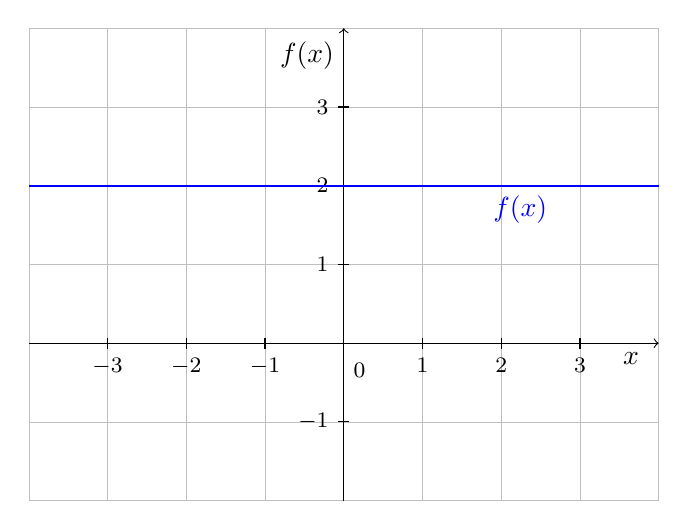
\begin{tikzpicture}
	
	% Gitternetzlinien
	\draw[xstep=1cm, ystep=1cm, very thin, color=lightgray] (-4,4) grid (4,-2);
	% x-Achse
	\draw[->] (-4,0) -- (4,0) node[below,xshift=-1em] {$x$}; 
	%Zahlen auf x-Achse
	\foreach \x in {-3,...,-1}
	\draw[shift={(\x,0)},color=black] (0pt,2pt) -- (0pt,-2pt) node[below] {\footnotesize $\x$};
	\foreach \x in {1,...,3}
	\draw[shift={(\x,0)},color=black] (0pt,2pt) -- (0pt,-2pt) node[below] {\footnotesize $\x$};
	% y-Achse 
	\draw[->] (0,-2) -- (0,4) node[left,yshift=-1em] {$f(x)$};%node[above left]
	%Zahlen auf y-Achse
	\foreach \y in {-1,...,-1}
	\draw[shift={(0,\y)},color=black] (2pt,0pt) -- (-2pt,0pt) node[left] {\footnotesize $\y$};
	\foreach \y in {1,...,3}
	\draw[shift={(0,\y)},color=black] (2pt,0pt) -- (-2pt,0pt) node[left] {\footnotesize $\y$};
	%Ursprung
	\draw[color=black] (0pt,-10pt) node[right] {\footnotesize $0$};
	
	\draw[thick,color=blue] plot[samples=200, domain=-4:4] 
	(\x,{2}) node[below, xshift=-5em] {$f(x)$};
	
	
	
	
	\end{tikzpicture}\\
\end{center}
\begin{center}
	\begin{align*}
	f:[-2,2]\longmapsto[-2,2]\;\;\text{mit }\;\;f(x)=x
	\end{align*}
	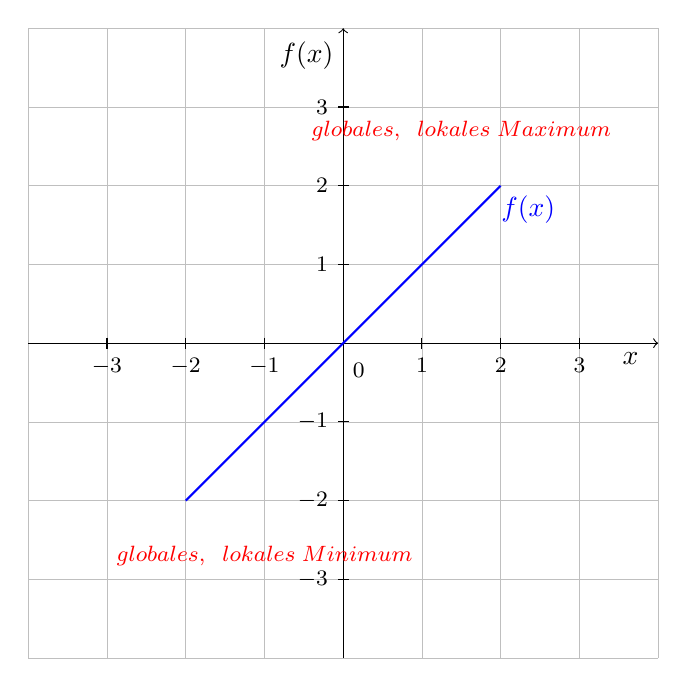
\begin{tikzpicture}
	
	% Gitternetzlinien
	\draw[xstep=1cm, ystep=1cm, very thin, color=lightgray] (-4,4) grid (4,-4);
	% x-Achse
	\draw[->] (-4,0) -- (4,0) node[below,xshift=-1em] {$x$}; 
	%Zahlen auf x-Achse
	\foreach \x in {-3,...,-1}
	\draw[shift={(\x,0)},color=black] (0pt,2pt) -- (0pt,-2pt) node[below] {\footnotesize $\x$};
	\foreach \x in {1,...,3}
	\draw[shift={(\x,0)},color=black] (0pt,2pt) -- (0pt,-2pt) node[below] {\footnotesize $\x$};
	% y-Achse 
	\draw[->] (0,-4) -- (0,4) node[left,yshift=-1em] {$f(x)$};%node[above left]
	%Zahlen auf y-Achse
	\foreach \y in {-1,...,-3}
	\draw[shift={(0,\y)},color=black] (2pt,0pt) -- (-2pt,0pt) node[left] {\footnotesize $\y$};
	\foreach \y in {1,...,3}
	\draw[shift={(0,\y)},color=black] (2pt,0pt) -- (-2pt,0pt) node[left] {\footnotesize $\y$};
	%Ursprung
	\draw[color=black] (0pt,-10pt) node[right] {\footnotesize $0$};
	
	
	
	\draw[thick,color=blue] plot[samples=200, domain=-2:2] 
	(\x,{\x}) node[below, xshift=1em]{$f(x)$};
	
	\draw[color=red] (-1,-2.7) node {\footnotesize $globales,\;\;lokales\; Minimum$};
	\draw[color=red] (1.5,2.7) node {\footnotesize $globales,\;\;lokales\; Maximum$};
	\end{tikzpicture}\\
\end{center}
\pagebreak
\begin{center}
	\begin{align*}
	f:]-2,2]\longmapsto\;]-2,2]\;\;\text{mit }\;\;f(x)=x
	\end{align*}
	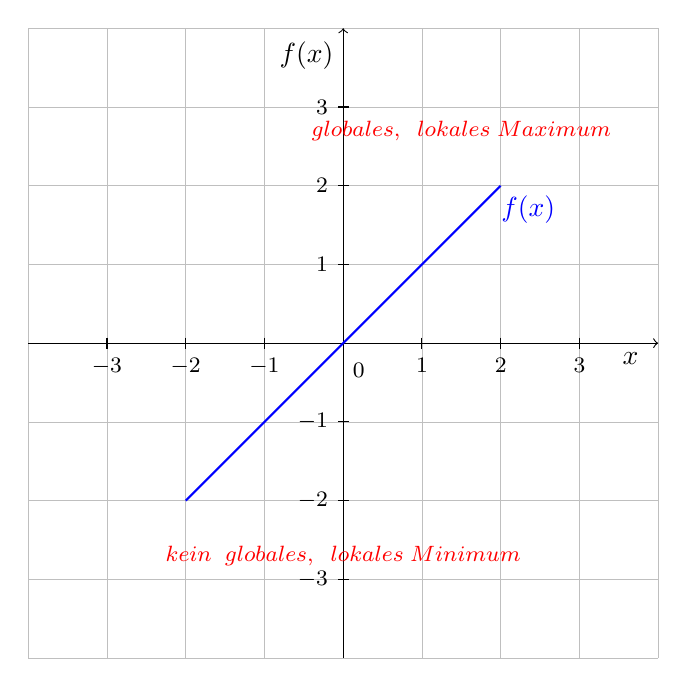
\begin{tikzpicture}
	
	% Gitternetzlinien
	\draw[xstep=1cm, ystep=1cm, very thin, color=lightgray] (-4,4) grid (4,-4);
	% x-Achse
	\draw[->] (-4,0) -- (4,0) node[below,xshift=-1em] {$x$}; 
	%Zahlen auf x-Achse
	\foreach \x in {-3,...,-1}
	\draw[shift={(\x,0)},color=black] (0pt,2pt) -- (0pt,-2pt) node[below] {\footnotesize $\x$};
	\foreach \x in {1,...,3}
	\draw[shift={(\x,0)},color=black] (0pt,2pt) -- (0pt,-2pt) node[below] {\footnotesize $\x$};
	% y-Achse 
	\draw[->] (0,-4) -- (0,4) node[left,yshift=-1em] {$f(x)$};%node[above left]
	%Zahlen auf y-Achse
	\foreach \y in {-1,...,-3}
	\draw[shift={(0,\y)},color=black] (2pt,0pt) -- (-2pt,0pt) node[left] {\footnotesize $\y$};
	\foreach \y in {1,...,3}
	\draw[shift={(0,\y)},color=black] (2pt,0pt) -- (-2pt,0pt) node[left] {\footnotesize $\y$};
	%Ursprung
	\draw[color=black] (0pt,-10pt) node[right] {\footnotesize $0$};
	
	
	
	\draw[thick,color=blue] plot[samples=200, domain=-2:2] 
	(\x,{\x}) node[below, xshift=1em]{$f(x)$};
	
	\draw[color=red] (0,-2.7) node {\footnotesize $kein\;\; globales,\;\;lokales\; Minimum$};
	\draw[color=red] (1.5,2.7) node {\footnotesize $globales,\;\;lokales\; Maximum$};
	\end{tikzpicture}\\
\end{center}
\subsection{ Extrema stetiger Funktionen}
\href{https://youtu.be/mIDbM-qesZs}{Video 13}\\
\underline{Satz}\\
Seien $ a,b\in\mathbb{R} $ und $ f:[a,b] \longmapsto \mathbb{W}_f\subseteq \mathbb{R}$, so besitzt $ f $ ein Maximum und ein Minimum.\vspace*{2mm}\\
Wenn eine stetige Funktion mit einem kompakten Intervall definiert ist, dann hat es mindestens ein Minumum und mindestens ein Maximum.\vspace*{2mm}\\
Beispiel:\\
$\blacktriangleright \;\; f:[-2,2] $ mit $ x \longmapsto x $\\
\begin{quote}
	Da $ f $ stetig ist und $[-2,2]  $ ein kompaktes Intervall besitzt hat die Funktion ein Maximum und ein Minimum.\\
	
	\pagebreak
	\begin{center}
		\begin{align*}
		f:[-2,2]\longmapsto\;[-2,2]\;\;\text{mit }\;\;f(x)=x
		\end{align*}
		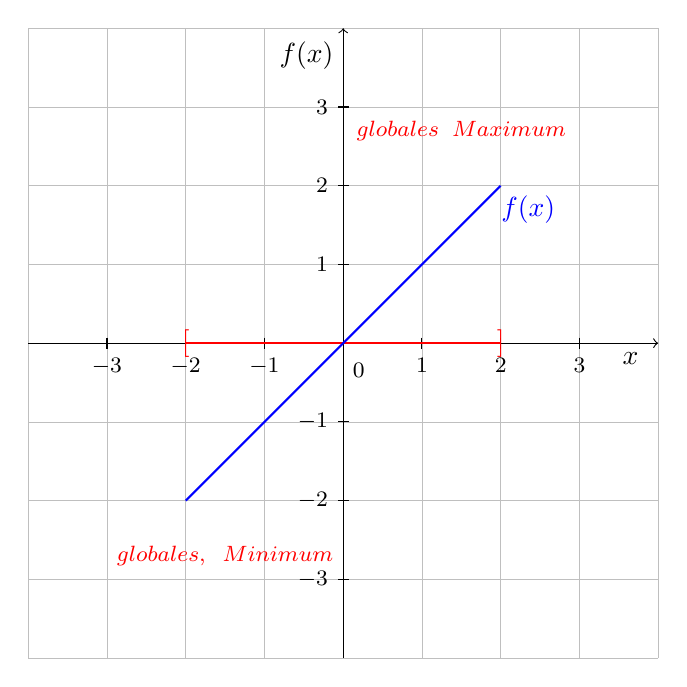
\begin{tikzpicture}
		
		% Gitternetzlinien
		\draw[xstep=1cm, ystep=1cm, very thin, color=lightgray] (-4,4) grid (4,-4);
		% x-Achse
		\draw[->] (-4,0) -- (4,0) node[below,xshift=-1em] {$x$}; 
		%Zahlen auf x-Achse
		\foreach \x in {-3,...,-1}
		\draw[shift={(\x,0)},color=black] (0pt,2pt) -- (0pt,-2pt) node[below] {\footnotesize $\x$};
		\foreach \x in {1,...,3}
		\draw[shift={(\x,0)},color=black] (0pt,2pt) -- (0pt,-2pt) node[below] {\footnotesize $\x$};
		% y-Achse 
		\draw[->] (0,-4) -- (0,4) node[left,yshift=-1em] {$f(x)$};%node[above left]
		%Zahlen auf y-Achse
		\foreach \y in {-1,...,-3}
		\draw[shift={(0,\y)},color=black] (2pt,0pt) -- (-2pt,0pt) node[left] {\footnotesize $\y$};
		\foreach \y in {1,...,3}
		\draw[shift={(0,\y)},color=black] (2pt,0pt) -- (-2pt,0pt) node[left] {\footnotesize $\y$};
		%Ursprung
		\draw[color=black] (0pt,-10pt) node[right] {\footnotesize $0$};
		
		\draw[color=red,thick] (-2,0)--(2,0);
		\draw[color=red,thick] (2,0) node {]};
		\draw[color=red,thick] (-2,0) node {[};
		\draw[thick,color=blue] plot[samples=200, domain=-2:2] 
		(\x,{\x}) node[below, xshift=1em]{$f(x)$};
		
		\draw[color=red] (-1.5,-2.7) node {\footnotesize $globales,\;\; Minimum$};
		\draw[color=red] (1.5,2.7) node {\footnotesize $globales\;\; Maximum$};
		\end{tikzpicture}\\
	\end{center}
\end{quote}
$\blacktriangleright \;\; f:[-2,2] $ mit $ x \longmapsto 1 $\\
\begin{quote}
	Jeder Punkt nimmt globales bzw. lokales Max./Min. ein.\\	
	\begin{center}
		
		\begin{align*}
		f:[-2,2]\longmapsto\;[1]\;\;\text{mit }\;\;f(x)=1
		\end{align*}
		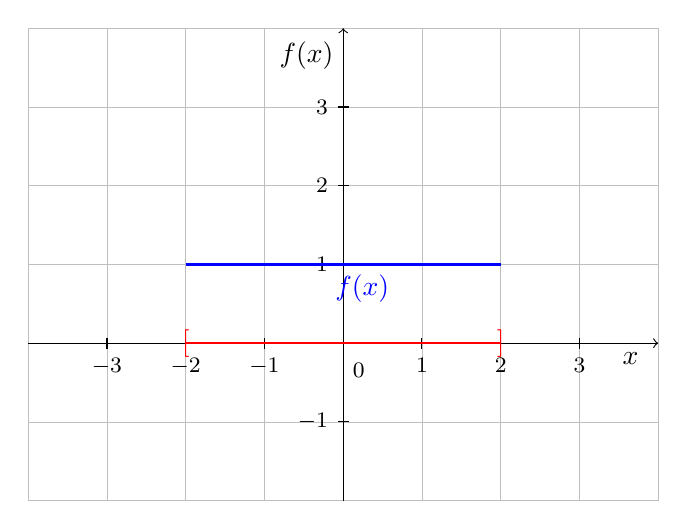
\begin{tikzpicture}
		
		% Gitternetzlinien
		\draw[xstep=1cm, ystep=1cm, very thin, color=lightgray] (-4,4) grid (4,-2);
		% x-Achse
		\draw[->] (-4,0) -- (4,0) node[below,xshift=-1em] {$x$}; 
		%Zahlen auf x-Achse
		\foreach \x in {-3,...,-1}
		\draw[shift={(\x,0)},color=black] (0pt,2pt) -- (0pt,-2pt) node[below] {\footnotesize $\x$};
		\foreach \x in {1,...,3}
		\draw[shift={(\x,0)},color=black] (0pt,2pt) -- (0pt,-2pt) node[below] {\footnotesize $\x$};
		% y-Achse 
		\draw[->] (0,-2) -- (0,4) node[left,yshift=-1em] {$f(x)$};%node[above left]
		%Zahlen auf y-Achse
		\foreach \y in {-1,...,-1}
		\draw[shift={(0,\y)},color=black] (2pt,0pt) -- (-2pt,0pt) node[left] {\footnotesize $\y$};
		\foreach \y in {1,...,3}
		\draw[shift={(0,\y)},color=black] (2pt,0pt) -- (-2pt,0pt) node[left] {\footnotesize $\y$};
		%Ursprung
		\draw[color=black] (0pt,-10pt) node[right] {\footnotesize $0$};
		
		\draw[thick,color=blue] plot[samples=200, domain=-2:2] 
		(\x,{1}) node[below, xshift=-5em] {$f(x)$};
		
		\draw[color=red,thick] (-2,0)--(2,0);
		\draw[color=red,thick] (2,0) node {]};
		\draw[color=red,thick] (-2,0) node {[};
		
		
		\end{tikzpicture}\\
	\end{center}
\end{quote}
$\blacktriangleright \;\; f:[-1,0[ $ mit $ x \longmapsto \frac{1}{x} $\\
\begin{quote}
	Hat ein globales Maximum und kein Minimum.\\
	\pagebreak
	
	\begin{center}
		
		\begin{align*}
		f:]-1,0[\;\longmapsto\;]-1,-\infty[\;\;\text{mit }\;\;f(x)=\frac{1}{x}
		\end{align*}
		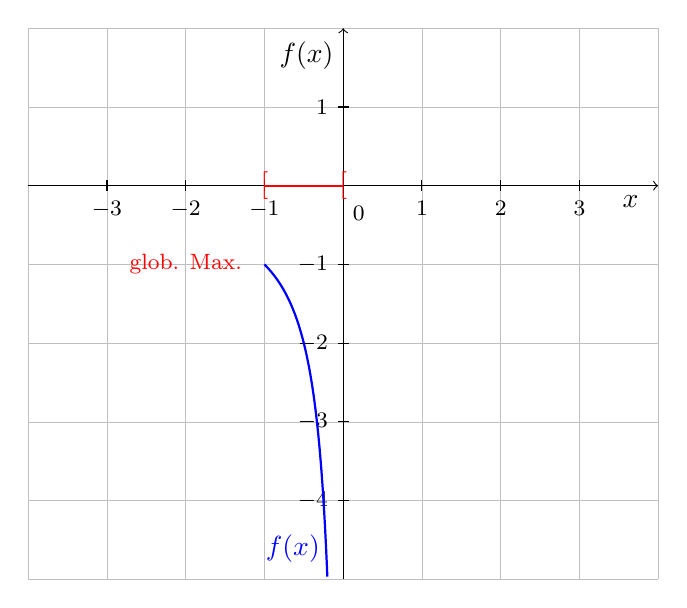
\begin{tikzpicture}
		
		% Gitternetzlinien
		\draw[xstep=1cm, ystep=1cm, very thin, color=lightgray] (-4,2) grid (4,-5);
		% x-Achse
		\draw[->] (-4,0) -- (4,0) node[below,xshift=-1em] {$x$}; 
		%Zahlen auf x-Achse
		\foreach \x in {-3,...,-1}
		\draw[shift={(\x,0)},color=black] (0pt,2pt) -- (0pt,-2pt) node[below] {\footnotesize $\x$};
		\foreach \x in {1,...,3}
		\draw[shift={(\x,0)},color=black] (0pt,2pt) -- (0pt,-2pt) node[below] {\footnotesize $\x$};
		% y-Achse 
		\draw[->] (0,-5) -- (0,2) node[left,yshift=-1em] {$f(x)$};%node[above left]
		%Zahlen auf y-Achse
		\foreach \y in {-1,...,-4}
		\draw[shift={(0,\y)},color=black] (2pt,0pt) -- (-2pt,0pt) node[left] {\footnotesize $\y$};
		\foreach \y in {1,...,1}
		\draw[shift={(0,\y)},color=black] (2pt,0pt) -- (-2pt,0pt) node[left] {\footnotesize $\y$};
		%Ursprung
		\draw[color=black] (0pt,-10pt) node[right] {\footnotesize $0$};
		
		\draw[thick,color=blue] plot[samples=200, domain=-1:-0.2] 
		(\x,{1/ \x}) node[left, xshift=1, yshift=10] {$f(x)$};
		
		\draw[color=red,thick] (-1,0)--(0,0);
		\draw[color=red,thick] (0,0) node {[};
		\draw[color=red,thick] (-1,0) node {[};
		\draw[color=red,thick] (-2,-1) node {\footnotesize glob. Max.};
		
		\end{tikzpicture}\\
	\end{center}
\end{quote}
Kein Minimum weil:\\
\begin{align*}
\lim\limits_ {\substack{x \to 0 \\ x<0}}\frac{1}{x}=-\infty\;\;\text{es existiert kein Minimum }
\end{align*}
Maximum weil:\\
\begin{align*}
\text{ Maximum ist bei} \;\;x_0=-1
\end{align*}
$\blacktriangleright \;\; f:]-1,0[ $ mit $ x \longmapsto \frac{1}{x} $\\
\begin{quote}
	Hat kein globales Maximum und kein Minimum.\\
	%\pagebreak
	
	\begin{center}
		
		\begin{align*}
		f:]-1,0[\;\longmapsto\;]-1,-\infty[\;\;\text{mit }\;\;f(x)=\frac{1}{x}
		\end{align*}
		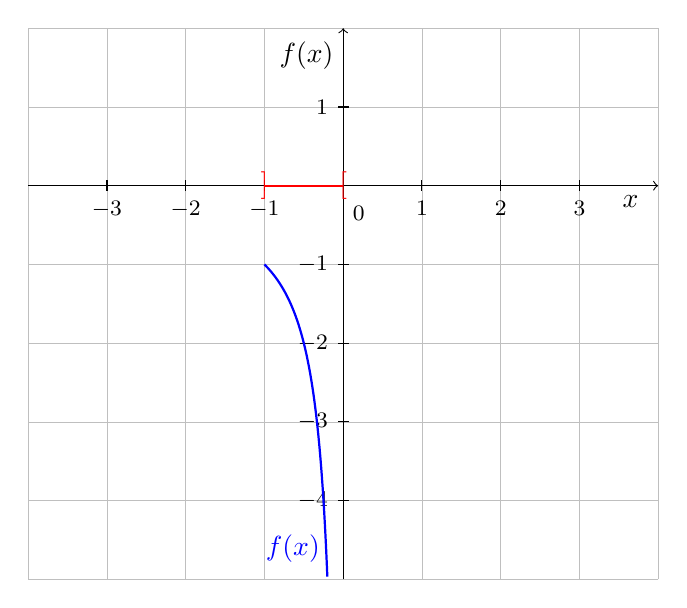
\begin{tikzpicture}
		
		% Gitternetzlinien
		\draw[xstep=1cm, ystep=1cm, very thin, color=lightgray] (-4,2) grid (4,-5);
		% x-Achse
		\draw[->] (-4,0) -- (4,0) node[below,xshift=-1em] {$x$}; 
		%Zahlen auf x-Achse
		\foreach \x in {-3,...,-1}
		\draw[shift={(\x,0)},color=black] (0pt,2pt) -- (0pt,-2pt) node[below] {\footnotesize $\x$};
		\foreach \x in {1,...,3}
		\draw[shift={(\x,0)},color=black] (0pt,2pt) -- (0pt,-2pt) node[below] {\footnotesize $\x$};
		% y-Achse 
		\draw[->] (0,-5) -- (0,2) node[left,yshift=-1em] {$f(x)$};%node[above left]
		%Zahlen auf y-Achse
		\foreach \y in {-1,...,-4}
		\draw[shift={(0,\y)},color=black] (2pt,0pt) -- (-2pt,0pt) node[left] {\footnotesize $\y$};
		\foreach \y in {1,...,1}
		\draw[shift={(0,\y)},color=black] (2pt,0pt) -- (-2pt,0pt) node[left] {\footnotesize $\y$};
		%Ursprung
		\draw[color=black] (0pt,-10pt) node[right] {\footnotesize $0$};
		
		\draw[thick,color=blue] plot[samples=200, domain=-1:-0.2] 
		(\x,{1/ \x}) node[left, xshift=1, yshift=10] {$f(x)$};
		
		\draw[color=red,thick] (-1,0)--(0,0);
		\draw[color=red,thick] (0,0) node {[};
		\draw[color=red,thick] (-1,0) node {]};
		%\draw[color=red,thick] (-2,-1) node {\footnotesize glob. Max.};
		
		\end{tikzpicture}\\
	\end{center}
	
	Kein Minimum weil:\\
	\begin{align*}
	\lim\limits_ {\substack{x \to 0 \\ x<0}}\frac{1}{x}=-\infty\;\;\text{es existiert kein Minimum }
	\end{align*}
	Kein Maximum weil:\\
	\begin{quote}
		
		\begin{align*}
		\lim\limits_ {\substack{x \to -1 \\ x>-1}}\frac{1}{x}=-1
		\end{align*}
		Aber $ -1\neq \mathbb{W}_f $ , deshalb existiert kein Maximun.\\
	\end{quote}
\end{quote}
\subsubsection{Aufgabe zu Extrema stetiger Funktionen}
\href{https://youtu.be/CkySz6nT0R8}{Video 14}\\
Haben folgende Funktionen globale Extrema?\\
(i)\;\;$ f:[2,17]\longmapsto \mathbb{R} $ mit $ f(x)=\frac{2x}{\mathrm{e}^x}-\cos(x) $\vspace*{2mm}\\
(ii)\;$ g:]0,1[\;\cup\;]1,2]\longmapsto \mathbb{R} $ mit $ g(x)= \frac{12}{1-x} $\vspace*{2mm}\\
zu (i):\\
\begin{quote}
	Die Funktion $ f $ ist als Komposition stetiger Funktionen in dem kompakten Intervall $[2,17]  $ stetig, also hat $ f $ ein globales Maximum und globales Minimum.
\end{quote}
zu (ii):\\
\begin{quote}
	Betrachte einseitige Grenzwerte:\\
	\begin{align*}
	\lim\limits_ {\substack{x \to 1 \\ x<1}}g(x)=\lim\limits_ {\substack{x \to 1 \\ x<1}} \frac{12}{1-x}=\infty
	\end{align*}
	Wenn $ x $ gegen 1 geht wird der Nenner ganz klein und der Bruch geht in das Unendliche.\\$ \Rightarrow $kein globales Maximum.
	\begin{align*}
	\lim\limits_ {\substack{x \to 1 \\ x>1}}g(x)=\lim\limits_ {\substack{x \to 1 \\ x>1}} \frac{12}{1-x}=-\infty
	\end{align*}
	Wenn $ x $ gegen gößer 1 zu 1 geht wird der Nenner negativ und ganz klein und der Bruch geht dannn in das negative Unendliche.\\
	$\Rightarrow $ kein globales Minimum.
\end{quote}
\subsection{Infimum und Supremum}
\href{https://youtu.be/z6nV00vtIVY}{Video 15}\\
\underline{Definition:}\\
Sei $ f:\mathbb{D}_f\longmapsto \mathbb{W}_f $ eine Funktion, $ x_0\in \mathbb{D}_f $ sowie $ y_0\in \mathbb{W}_f\cup \{+\infty\} $ (bzw.$ \mathbb{W}_f\cup \{-\infty\} $).\vspace*{2mm}\\
$ y_0 $ heißt Supremum (bzw. Infimum) von $ f $, wenn gilt:\\
(i) \;$ f(x)\leq y_0 $ (bzw. $ f(x) \geq y_0$) für alle $ x\in\mathbb{D}_f $\\
(ii) Es gibt eine Folge $ (x_n)_{n\in\mathbb{N}} $ mit $ \lim\limits_ {n\to\infty}=y_0$\vspace*{2mm}\\
Man schreibt dann:\\
\begin{align*}
\sup_{x\in\mathbb{D}_f}=y_0\\
\inf_{x\in\mathbb{D}_f}=y_0
\end{align*}
Beispiel:\\
(i) $ f:\mathbb{R}\longmapsto [0,\infty[ $ mit $f(x)=x^2$
\begin{quote}
	\textbullet \;\; $ \underset{x\in\mathbb{R}}{\sup}f(x)=\infty $ wegen $ \lim\limits_ {x\to\infty}f(x) =\infty$\\
	\textbullet	\;\; $ \underset{x\in\mathbb{R}}{\inf}f(x)=0 $ \;\;\;\; ist auch ein globales Minimum\\
\end{quote}
\begin{center}
	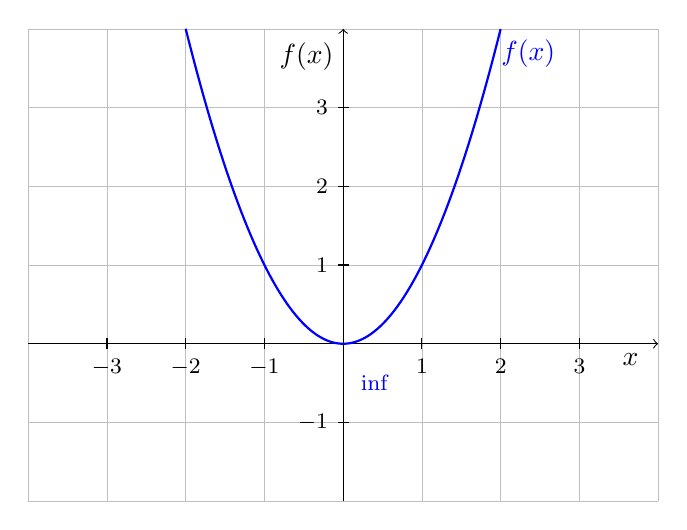
\begin{tikzpicture}
	
	% Gitternetzlinien
	\draw[xstep=1cm, ystep=1cm, very thin, color=lightgray] (-4,4) grid (4,-2);
	% x-Achse
	\draw[->] (-4,0) -- (4,0) node[below,xshift=-1em] {$x$}; 
	%Zahlen auf x-Achse
	\foreach \x in {-3,...,-1}
	\draw[shift={(\x,0)},color=black] (0pt,2pt) -- (0pt,-2pt) node[below] {\footnotesize $\x$};
	\foreach \x in {1,...,3}
	\draw[shift={(\x,0)},color=black] (0pt,2pt) -- (0pt,-2pt) node[below] {\footnotesize $\x$};
	% y-Achse 
	\draw[->] (0,-2) -- (0,4) node[left,yshift=-1em] {$f(x)$};%node[above left]
	%Zahlen auf y-Achse
	\foreach \y in {-1,...,-1}
	\draw[shift={(0,\y)},color=black] (2pt,0pt) -- (-2pt,0pt) node[left] {\footnotesize $\y$};
	\foreach \y in {1,...,3}
	\draw[shift={(0,\y)},color=black] (2pt,0pt) -- (-2pt,0pt) node[left] {\footnotesize $\y$};
	%Ursprung
	%\draw[color=black] (0pt,-10pt) node[right] {\footnotesize $0$};
	
	
	\draw[thick,color=blue] plot[samples=200, domain=-2:2] 
	(\x,{\x*\x}) node[below, xshift=1em]{$f(x)$};
	\draw[color=blue] (0.1,-0.5) node[right] {\footnotesize $\inf$};
	
	
	\end{tikzpicture}\\
\end{center}
(ii)\;\;$ f:\mathbb{R}\backslash\{0\} \longmapsto \mathbb{R}$ mit $ f(x)=\frac{1}{x} $\\
\begin{quote}
	\textbullet \;\;$ \underset{x\in \mathbb{R}\backslash\{0\}}{\sup} f(x)=\infty$ wegen $ \lim\limits_ {\substack{x \to 0\\x>0}}\frac{1}{x}=\infty $\\
	\textbullet \;\; $\underset{x\in \mathbb{R}\backslash\{0\}}{\inf} f(x)=-\infty$ wegen $ \lim\limits_ {\substack{x \to 0\\x<0}}\frac{1}{x}=-\infty $\\
\end{quote}
\begin{center}
	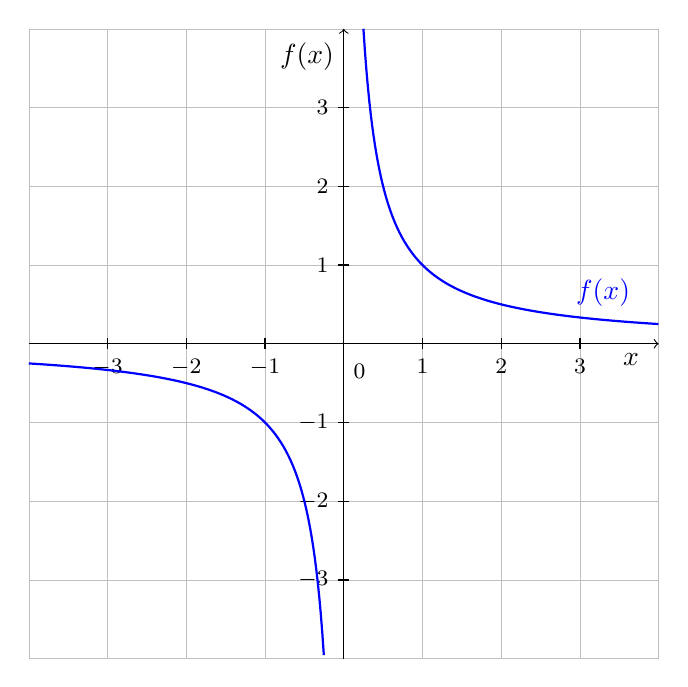
\begin{tikzpicture}
	
	% Gitternetzlinien
	\draw[xstep=1cm, ystep=1cm, very thin, color=lightgray] (-4,4) grid (4,-4);
	% x-Achse
	\draw[->] (-4,0) -- (4,0) node[below,xshift=-1em] {$x$}; 
	%Zahlen auf x-Achse
	\foreach \x in {-3,...,-1}
	\draw[shift={(\x,0)},color=black] (0pt,2pt) -- (0pt,-2pt) node[below] {\footnotesize $\x$};
	\foreach \x in {1,...,3}
	\draw[shift={(\x,0)},color=black] (0pt,2pt) -- (0pt,-2pt) node[below] {\footnotesize $\x$};
	% y-Achse 
	\draw[->] (0,-4) -- (0,4) node[left,yshift=-1em] {$f(x)$};%node[above left]
	%Zahlen auf y-Achse
	\foreach \y in {-3,...,-1}
	\draw[shift={(0,\y)},color=black] (2pt,0pt) -- (-2pt,0pt) node[left] {\footnotesize $\y$};
	\foreach \y in {1,...,3}
	\draw[shift={(0,\y)},color=black] (2pt,0pt) -- (-2pt,0pt) node[left] {\footnotesize $\y$};
	%Ursprung
	\draw[color=black] (0pt,-10pt) node[right] {\footnotesize $0$};
	
	\draw[thick,color=blue] plot[samples=200, domain=0.25:4] 
	(\x,{1/\x}) node[below, xshift=-2em,yshift=2em]{$f(x)$};
	
	\draw[thick,color=blue] plot[samples=200, domain=-4:-0.25] 
	(\x,{1/\x});
	
	
	
	\end{tikzpicture}\\	
\end{center}
\subsubsection{Aufgabe zu Infimum und Supremum}
\href{https://youtu.be/HnmGV8AtkOc}{Video 16}\\
Bestimme bei folgenden Funktionen das Infimum und Supremum.\vspace*{2mm}\\
(i)\;\;\;$ \tan:\; ]-\frac{\pi}{2},\frac{\pi}{2}[\;\;\longmapsto \mathbb{R} $ mit $ \tan(x)=\frac{\sin(x)}{\cos(x)} $\vspace*{2mm}\\
(ii)\; $ g:\mathbb{R}\backslash\{\pm 1\} \longmapsto \mathbb{R}$ mit $ g(x)=\frac{7x}{x^2-1} $\vspace*{2mm}\\
Zu (i):\\
\begin{quote}
	Skizze von Cosinus und Sinus:\\
	\begin{center}
		
		
		\begin{tikzpicture}[scale=2]
		
		% Gitternetzlinien
		\draw[xstep=1cm, ystep=1cm, very thin, color=lightgray] (-3.5,2) grid (3.5,-2);
		% x-Achse
		\draw[->] (-3.5,0) -- (3.5,0) node[below,xshift=-1em] {$x$}; 
		%Zahlen auf x-Achse
		\foreach \x in {-2,...,-1}
		\draw[shift={(\x,0)},color=black] (0pt,2pt) -- (0pt,-2pt) node[below] {\footnotesize $\x$};
		\foreach \x in {1,...,2}
		\draw[shift={(\x,0)},color=black] (0pt,2pt) -- (0pt,-2pt) node[below] {\footnotesize $\x$};
		% y-Achse 
		\draw[->] (0,-2) -- (0,2) node[left,yshift=-1em] {$f(x)$};%node[above left]
		%Zahlen auf y-Achse
		\foreach \y in {-1,...,-1}
		\draw[shift={(0,\y)},color=black] (2pt,0pt) -- (-2pt,0pt) node[left] {\footnotesize $\y$};
		\foreach \y in {1,...,1}
		\draw[shift={(0,\y)},color=black] (2pt,0pt) -- (-2pt,0pt) node[left] {\footnotesize $\y$};
		%Ursprung
		\draw[color=black] (0pt,-10pt) node[right] {\footnotesize $0$};
		
		\draw[thick,color=blue] plot[samples=200, domain=-3.5:3.5] 
		(\x,{sin(\x r)}) node[xshift=-1em,yshift=4.5em]{$\sin(x)$};
		\draw[thick,color=red] plot[samples=200, domain=-3.5:3.5] 
		(\x,{cos(\x r)}) node[xshift=1em,yshift=1.5em]{$\cos(x)$};
		\draw[color=green] (-3.14/2,-1.2) node {\footnotesize $-\genfrac{}{}{}{2}{\pi }{2 }$};
		\draw[color=green] (3.14/2,-1.2) node {\footnotesize $\genfrac{}{}{}{2}{\pi }{2 }$};
		\draw[color=green] (3.14/2,1)--(3.14/2,-1);
		\draw[color=green] (-3.14/2,1)--(-3.14/2,-1);
		\end{tikzpicture}\\
		
	\end{center}
	\textbullet \;\;$ \lim\limits_ {\substack{x \to \frac{\pi}{2}  \\ x< \frac{\pi}{2}}} \tan(x)=\lim\limits_ {\substack{x \to \frac{\pi}{2}  \\ x< \frac{\pi}{2}}}\frac{\sin(x)}{\cos(x)}=+\infty $\\
	\begin{quote}
		Bemerkung: $ +\infty $, weil der Zähler bei $ \frac{\pi}{2}$ positiv ist, wenn der $ \cos(\frac{\pi}{2}) $ Null wird.\\
		
		$\Rightarrow  \underset{x\in \mathbb{D}_f}{\sup}\tan(x) =+\infty $
		
	\end{quote}
	\textbullet \;\;$ \lim\limits_ {\substack{x \to -\frac{\pi}{2}  \\ x> -\frac{\pi}{2}}} \tan(x)=\lim\limits_ {\substack{x \to -\frac{\pi}{2}  \\ x> -\frac{\pi}{2}}}\frac{\sin(x)}{\cos(x)}=-\infty $\\
	\begin{quote}
		Bemerkung: $ -\infty $, weil der Zähler bei $ -\frac{\pi}{2}$ negativ ist, wenn der $ \cos(-\frac{\pi}{2}) $ Null wird.\\
		
		$\Rightarrow  \underset{x\in \mathbb{D}_f}{\inf}\tan(x) =-\infty $
		
	\end{quote}
	
\end{quote}
\pagebreak
Zu (ii):\\
\begin{quote}
	\textbullet\;\; $\lim\limits_ {\substack{x \to 1 \\ x>1}}g(x)=\lim\limits_ {\substack{x \to 1 \\ x>1}}\frac{7x}{x^2-1}=+\infty$\\
	\begin{quote}
		Bemerkung:$ +\infty $, weil Nenner negativ bei $ x>1 $wird und der Zähler durch 7 beschränkt ist  und positiv ist.\\
		$\Rightarrow  \underset{x\in \mathbb{D}_f}{\sup}g(x) =+\infty $
		
	\end{quote}
	\textbullet\;\; $\lim\limits_ {\substack{x \to 1 \\ x<1}}g(x)=\lim\limits_ {\substack{x \to 1 \\ x<1}}\frac{7x}{x^2-1}=-\infty$\\
	\begin{quote}
		Bemerkung:$ -\infty $, weil Nenner negativ bei $ x<1 $wird und der Zähler durch 7 beschränkt ist  und positiv ist.\\
		$\Rightarrow  \underset{x\in \mathbb{D}_f}{\inf}g(x) =-\infty $
		
	\end{quote}
	Den Fall für -1 braucht man ja nicht mehr zu betrachten, weil schon ein Infimum um Supremum gefunden wurde.\\
\end{quote}